\documentclass[a4paper,12pt, oneside]{memoir}

\usepackage{csvsimple}
\usepackage{lipsum}
\usepackage{listings}
\usepackage{color}

\definecolor{dkgreen}{rgb}{0,0.6,0}
\definecolor{gray}{rgb}{0.5,0.5,0.5}
\definecolor{mauve}{rgb}{0.58,0,0.82}

\lstset{frame=tb,
  language=Java,
  aboveskip=3mm,
  belowskip=3mm,
  showstringspaces=false,
  columns=flexible,
  basicstyle={\small\ttfamily},
  numbers=none,
  numberstyle=\tiny\color{gray},
  keywordstyle=\color{blue},
  commentstyle=\color{dkgreen},
  stringstyle=\color{mauve},
  breaklines=true,
  breakatwhitespace=true,
  tabsize=3
}
\usepackage{wrapfig}
\usepackage{titlesec}
\titleformat{\chapter}[display]
{\normalfont\huge\bfseries}{}{0pt}{\Huge}
\titlespacing*{\chapter} {0pt}{0pt}{15pt}
\usepackage{algpseudocode,algorithm}
\usepackage{multicol}
\usepackage{diagbox,booktabs,amsmath}
\usepackage{graphicx}
\usepackage{cite}
\graphicspath{ {images/} }
\usepackage[utf8]{inputenc}
\usepackage{hyperref} % hyperlinks
\usepackage{url}
\usepackage{caption}
\usepackage{subcaption}
\usepackage{amsmath}
\usepackage{txfonts}
\usepackage{geometry} % all margins
 \geometry{
   a4paper,
   total={210mm,297mm},
   left=13mm,
   right=13mm,
   top=15mm,
   bottom=15mm,
 }

\begin{document}

\title{A Comparison of Algorithms for Coevolving The Weights and Topologies of Artificial Neural Networks.}
\author{Hichame Moriceau\\
  Computing Science Honours project\\ \\
  School of Computing,\\
  Edinburgh Napier University,\\
  10 Colinton Road,\\
  United Kingdom,\\
  EH10 5DT\\}
\date{\today}
\maketitle

\begin{abstract}
Artificial Neural Networks (ANNs) are a very popular method used for classification problems. Today, the combination of gradient descent with the backpropagation algorithm is the most popular alternative used for training ANNs. Using this method implies that an analyst must manually find the most adequate topology for the problem at hand however, more adaptive methods can be used to to automate this process. In this dissertation, the use of population-based evolutionary algorithms such as Differential Evolution (DE) and Particle Swarm Optimization (PSO) is investigated as ways to autonomously find a most adequate combination of architecture and weights. DE is a simple and powerful stochastic evolutionary algorithm successfuly applied to a variety of problems in the past. PSO is a more recent stochastic algorithm inspired by the social behaviour of flock of birds and schools of fish. DE and PSO are used independently for training ANNs on the breast cancer malignance problem, the breast cancer recurrence problem and the Haberman's suvival problem. Both DE and PSO have been used in the past as ways to train the weights of ANNs and more recently to coevolve their topology and weights. The experiment shows that results approaching the state-of-the-art are achieved using DE and that the canonical PSO algorithm produces a very fast search with a tendency to get stuck at a local optima. An observation of the ability of the population to be used as an ensemble is made. Finally, some important conclusions and potential research path are suggested.
\end{abstract}

\clearpage

\tableofcontents

\clearpage
\chapter{Acknowledgements}
Many thanks to Prof Simon Powers for having been the main supervisor of this research project. The relevance and quality of his comments always led me to challenge myself and explore interesting paths. Our discussions nourished my reflection and helped me validate my results. I cannot emphasize enough how much I look forward to pursue this collaboration in the context of a future research internship.
\\ \\
Thanks to Prof Neil Urquhart for his advice and guidance as the initial supervisor of this project. I would also thank him for the key insights I gained about the combination of global/local search and the theory around Evolutionary Computation in the context of the \textit{Computational Intelligence} class.
\\ \\
Thanks to Prof Eduardo Segredo for recommending me to work with Differential Evolution when a traditional Genetic Algorithm appeared to be a destructive method, a key insight that led me to achieve one of the main milestones of this project.
\\ \\
Thanks to Prof Kevin Sim for his great insights on hyper-heuristics, our discussions helped me choose the most appropriate path to explore within these vast subjects that are Machine Learning and Biology-Inspired Computing.
\\ \\
Thanks to Edinburgh Napier University to let students access online publications. Justifying the interest and relevance of this topic would have been much more difficult without the ability to use resources such as IEEExplore.
\\ \\
This project would not have been possible without all the resources available on The Internet. Specifically Andrew Ng's wonderful Stanford online course on machine learning which taught me a lot about Data Science as well as the math behind Artificial Neural Networks. I would also like to thank the open source community to publicly share their work. Without the existence of the community, this project would not have been so interesting. Finding open resources whether it is free software such as GNU Octave that I used to print my results, open data sets such as the Machine Learning UCI data set repository or being able to compare my algorithms implementations with other functional ones in other languages on Github or even open publications on ArXiv tremendously facilitated my progress.

\chapter{Introduction}

\section{Motivations}

Over the last few years we have observed Artificial Intelligence technologies being used in an increasingly vast range of industries going from trading systems to face recognition, also medical diagnosis or even autonomous driving. The versatility of Neural Networks recently led to the emergence of \textit{Deep Learning}, a term that refers to the use of Neural Networks (typically Deep Neural Networks or Convolutional Networks\cite{lecun-convolutional-2010}). Neural Networks is an exceedingly relevant topic, recently, Deep Convolutional Networks were at the origin of a historic A.I. breakthrough: the first machine beating a world class expert at the game of 'Go' \cite{hassabis-2016}.
\\ \\
To this day, a multitude of pattern-recognition approaches exist. From the simple Linear Regression to more complex model classes like Support Vector Machines, it is known that certain codel classes are best suited to specific types of problems. It is also known from the No-Free-Lunch theorem that there is no generic learning algorithm that outperforms problem-specific learning algorithms. In fact, in order to develop a predictive system for a given scenario, traditionally a data analyst would perform what is called \textit{feature engineering}. During this phase the analyst - by means of thinking and trying - would investigate what are considered the most interesting attributes as well as the most suitable model architecture. It was originally one of the goals of Yann Lecun to use Neural Networks to automate this process\cite{lecun-data-driven-2014}. By doing so, a fundamental architectural problem was solved. 
\\ \\
A valid argument for not taking the burden of building a Neural Network for learning a task is that it can be solved with a simpler model \cite{chilimbi-2014} \cite{huang-2013}. However, one of the purpose of researching adaptive methods is to find a method that will be good enough for the industry, whatever the problem at hand is. We have previously seen that thanks to the use of GPUs it is now practically possible to use neural networks for a wider range of problems. I believe that simple models are useful today because of the computational limit that we face but that as progress continues, these limits will be overcome and more adaptive and therefore more intelligent software will be usable by the industry for both simple and hard problems. The milestones achieved by the scientific community motivated me to investigate some of the existing methods developed to attain a narrow but highly adaptive A.I. 

\section{Scope}

This project is achieved by a single programmer in the context of a $4^{th}$ year full time Computing Science degree. This includes 2 other modules for each semester and a total of approximately 8 months to learn about machine learning, write the software, produce and validate interesting results and finally write this dissertation. I also take into account that it is proven extremely difficult to estimate the time required for any software engineering project. 
\\ \\
My interest will focus only on exploring how to use ANNs and algorithms such as evolutionary methods and swarm intelligence to solve three problems. Some much more complex algorithms such as the NEAT method \cite{stanley-2002} have been developed for evolving the topology and the weights of neural networks however implementing such a solution or building upon it has been considered out of the scope of this project.

\newpage

\section{Aims and Objectives} \label{section:aims-and-objectives}
Considering the context and scope of the project, the following milestones were identified.

\begin{multicols}{2}
  \begin{enumerate}
    \setlength\itemsep{0.001em}
    \item Find interesting data sets.
    \item Study Machine Learning techniques.
    \item Research already existing biology inspired techniques that independently evolve all parameters of a model.
    \item Implementing a neural network that can have any given topology.
    \item Implementing a traditional genetic algorithm.
    \item Implementing differential evolution (if necessary).
    \item Implementing particle swarm optimization (if possible).
    \item Implementing neural network ensembles (if possible).
    \item Implementing a benchmark application to validate and compare results.
    \item Writing the dissertation.
    \item Designing an A1 poster for presentating my results.
  \end{enumerate}
\end{multicols}

\subsection{Justifications}

It is known that to provide predictions with high generalization capabilities, it is important to pick a model according to the problem's complexity. Even though it is also known\cite{yao-1999} that in general, no single algorithm is an overall winner for all kinds of networks and that the best training algorithm is problem dependant. In the context of Neural Networks, this translates into the intuition that a Neural Network with a single hidden layer and few hidden units can only be trained successfully on simple tasks (e.g., boolean logic functions), while larger ANNs (i.e., Deep Belief Networks) can be successfully trained on more complex tasks (pattern recognition in images etc.) \cite{haykin-1998}. In other words, ANNs represent a solid candidate towards creating a \textit{generic}, \textit{adaptive} classifier, provided that the architecture is wisely selected. Just as for feature engineering, it is considered the job of the developer to find the best topology for a neural network. Contributing to developing an algorithm that automates this process in the context of \textit{supervised learning} is one of my main goals.
\\
\\
Considering the goal of this project, it is necessary to explore Neural Network architectures from the ground up. This requires investigating \textit{adaptive} machine learning algorithms that have been identified as having shown promising performances (Evolutionary Programming, Backpropagation). The intent of this work is not to produce the most accurate prediction for a given problem, but to build the system that is very much capable of learning a task with decent results. Therefore I am not just interested in applying a certain model to a certain problem. I am interested in experimenting with concepts from machine learning, biology-inspired computing and statistics in a coherent way to obtain a system that can adapt itself to different problems.

\section{Prerequisites}

This project required comprehension of the following concepts.

\begin{multicols}{2}
\begin{itemize}
  \setlength\itemsep{0.001em}
  \item Background in biology-inspired computing and machine learning
  \item Evolutionary algorithms \& Neural Networks
  \item Machine learning system design \& debugging methodology
  \item Linear algebra \& statistics (mean, median, variance, k-fold cross-validation etc.)
  \item Research methodology (literature investigation, reproducibility, benchmarking, questioning plots etc.)
  \item \textit{C++} \& \textit{Octave} programming
  \item Concurrency using \textit{OpenMP}
  \item Version Control using \textit{Git}
\end{itemize}
\end{multicols}

\newpage

\section{Structure of the Report}

The existing Neural Network and Evolutionary Programming algorithms found in the literature review will first be discussed. Secondly, the experimentation methodology and the design of the benchmark will be explained. The results obtained in the experiment will be presented along with an interpretation and a critical analysis. Finally, a conclusion will be drawn to assess the results of the project as well as its practical value.

\section{Terminology}

\begin{description}
     \setlength\itemsep{0.001em}
     \item  [Artificial Neural Networks] \hfill \\
      Also referred to as Neural Networks (ANNs) MultiLayer Perceptrons (MLP).
     \item  [Attributes] \hfill \\
      Is used alternatively with the word \textit{features} to refer to the \textit{characteristics} of the examples, whether they are of the type \textit{categorical}, \textit{ordinal} or \textit{numerical}.  
     \item  [Categorical] \hfill \\
      Designates the type of an attribute that is finite. Categorical attributes can be \textit{ordinal} ('Low', 'Medium', 'High') or non-ordinal ('Netherlands', 'United Kingdom', 'France'). \\
      Example: linear regression : $y = ax + b$.
     \item  [Class attribute] \hfill \\
      Is used alternatively with the word \textit{target attribute} to describe the attribute that contains the \textit{labels}.
     \item  [Data object] \hfill \\
      Is used alternatively with the words \textit{example}, \textit{instance} or \textit{field} to designate a single \textit{sample} in a data set.
     \item  [Generation] \hfill \\
      Is used alternatively with the word \textit{epoch} to describe a single iteration of optimization.
     \item  [Genetic Algorithms] \hfill \\
      Is used alternatively with its subtypes to designate algorithms inspired by evolution, specifying a crossover and a mutation operation. 
     \item  [Model] \hfill \\
      Is used to designate a specific solution belonging to a certain model class.
     \item  [Model class] \hfill \\
      Is used to designate the architecture of a model without specifying the values of its parameters. \\
      Example: linear regression : $y = 3x - 2$.
     \item  [Numerical] \hfill \\
      Designates the type of an attribute that is continuous. \\
      Example height in cm: 0, 1, 2 \dots 191, 192 \dots.
     \item  [Topology] \hfill \\
      Is used alternatively with the term \textit{architecture} in the context of neural networks.
    \item  [Score] \hfill \\
      Is used alternatively with the term \textit{fitness}. The term score is typically used in the field of machine learning whereas fitness relates to its equivalent in evolutionary computation.

\end{description}

\chapter{Literature Review}
This chapter evaluates the existing methods in terms of using neural networks as a way for solving different problems. This review goes through the logic behind EAs, ANNs and finally review several EA-based and swarm-intelligence-based techniques identified in the literature as promising ways to achieve a highly adaptive GANN.

\newpage

\section{Evolutionary Algorithms Theory}

\subsection{Background}
Genetic Algorithms (GAs) are a subtype of Evolutionary Algorithms (EAs) which also contains Evolution Strategies etc. All of which belong to the field of biology-inspired computing. A GA is a constructive search heuristic algorithm that mimics the process of natural selection. Inspired by Darwin's theory of evolution, a GA trains a superior population of solutions by breeding and mutating fittest individuals. In this experiment, a subtype of GA called \textit{Differential Evolution} will be used.
\\ \\
In order to implement a GA, two elements are required: a \textit{genome representation} and a \textit{fitness function}. The genome also refered as \textit{genotype} represents the primary description of a single solution and is traditionally expressed by a binary string although it is known from \cite{wikipedia-evolutionary-algorithms} that the best representations are usually those that reflect something about the problem being solved. The fitness function provides a single-valued metric to compare the quality of an individual (or solution) with another. By extension, good individuals are referred as fit and bad as unfit.

\setlength{\columnsep}{20pt}
\begin{wrapfigure}{r}{0.4\textwidth}
  \hspace{100pt}
  \begin{center}
    \includegraphics[scale=0.75]{GeneticAlgorithm}
  \end{center}
  \vspace{-20pt}
  \caption{Canonical Genetical Algorithm. Sources: \cite{haupt-1998} and \cite{negnevitsky-2011}.}
  \label{GA-flowchart}
\vspace{-40pt}
\end{wrapfigure}
\hspace{0pt}
\subsection{Logic description}

Figure \ref{GA-flowchart} illustrates the logic of a GA. Initially, a population of random solution is generated, then, the main loop is entered. This loop is constituted of 5 evolution phases. 
\\ \\
In the \textit{evaluation phase}, the fitness value of each individual is calculated, then, parents are chosen in the \textit{selection phase}. In the canonical elitist GA, only the two fittest individuals are selected as parents. The selected parents then produce an offspring, by means of a crossover operation to produce the new individual. The \textit{crossover phase} uses the genotypes of the selected parent to produce a novel combination of these. A wide variety of crossover operations exist (e.g., one or two point crossover, three parents crossover) Once generated, the offspring has a probability to be mutated. The \textit{mutation operation} is a minor random alteration of the genome.
\\ \\
This process is repeated until the fittest individual in the population satisfies a chosen criteria. Typically, this criteria will be a maximum number of generation or a convergence test (variance test).

\subsection{Search Space Behaviour}

Optimization algorithms can be classified in two categories, \textit{global search} and \textit{local search} algorithms. GAs belong to the former. Global search algorithms explore a broad spectrum of the search space whereas local search algorithms only exploit solutions that are near the current best solution. Typical example of local search algorithms are gradient based methods or neighborhood optimization techniques.
\\ \\ 
Being a global search algorithm, it has the advantage of having the tendency to converge towards the global optima. However, it is generally slower to converge as opposed to a local search algorithm.

\newpage

\section{Neural Network Theory}

% taken from wikipedia
% https://en.wikibooks.org/wiki/Artificial_Neural_Networks/Print_Version
\begin{figure}[!ht]
  \centering
  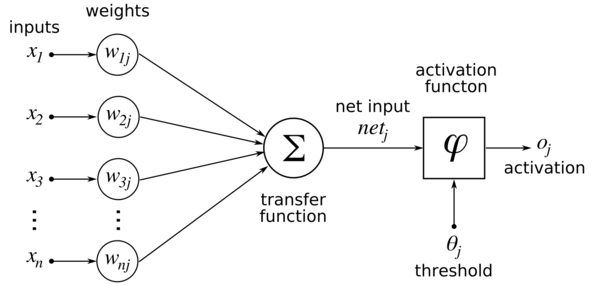
\includegraphics[scale=0.5] {ModelOfArtificialNeuron}
  \caption {Representation of a single artificial neuron. Source: \cite{wiki-artificial-neuron}}
  \label{single-neuron-diagram}
\end{figure}

As displayed by Figure \ref{neural-network-example} a neural network is composed of a multitude of artificial neurons, a neuron being the single computational unit of the network. A neural network comprises three main parts: \textit{the input layer}, a number of \textit{hidden layers} and the \textit{output layer}. 
\\ \\
Each neuron works in a very simple manner: firstly, multiple inputs are received from all previous neurons and added up. Following this, an activation function is applied to that value, and if that value exceeds that of a threshold, a signal is sent to the next layer. Figure \ref{single-neuron-diagram} and Formula \eqref{single-neuron-equation} illustrate this principle, where \textit{U} is the unactivated output of a neuron, $x_i$ is an input and $w_i$ its corresponding weight. 

\begin{equation} \label{single-neuron-equation}
  U_i = \sum_{j=1}^{n} x_i w_{ij} 
\end{equation}

The activation function is used to smoothly map varied range neuron-inputs onto a defined range (see \ref{sec:artificial-neural-network}). The range of the activation function can allow weights to express the positive or negative importance of a feature. The typical activation function used in neural networks is the sigmoid function. The logistic function can also be used in order to work with positive values only. Finally, the neuron has as many connections (formerly \textit{axons}) as the next layer has neurons. Each connection between one neuron and another holds a weight value. The weight values and the architecture of the network are the two main ways to train the network.

\subsection{Choice of the activation function}

Negnevitsky \cite{negnevitsky-2011} demonstrated that the hyperbolic tangent tends to deliver better results than other activation functions in that it leads to training a neural network with fewer epochs. Sibi \cite{sibi-2013} also experienced that using the Elliot function (higher speed approximation of hyperbolic tangeant) yields better results than the Sigmoid in the same respect but that the activation function was a less important criteria than the weights or the architecture of a network.

\subsection{Artificial Neural Networks}
\label{sec:artificial-neural-network}

\begin{quotation}
``Artificial neural network, a data mining practice, is an interconnected group of artificial neurons that uses mathematical model or computational model for information processing based on connectionnist approach of computation.'' Nilakshi P. Waghulde\cite{waghulde-2014}
\end{quotation}

In artificial intelligence, the term Artificial Neural Network refers to a learning model inspired by the brain. A typical application for an ANN is the handwritten digit recognition. In order to obtain a neural network able to recognize digits, the following process is executed. The weights are iteratively \textit{trained} so that, when feeding an image from the data set to the input of the network (one pixel per input neuron), the output neuron corresponding to the given digit is activated.

\begin{figure}[h]
  % taken from a post on stackexchange
  % http://tex.stackexchange.com/questions/132444/diagram-of-an-artificial-neural-network
  \begin{center}
    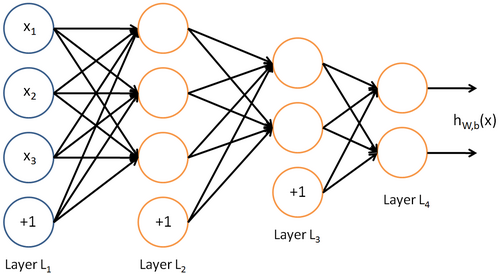
\includegraphics[scale=0.65]{neural-net-diagram}
  \end{center}
  \caption{Example of a fully connected ANN with two hidden layers and bias units (+1). Source: \cite{coursera-machine-learning-stanford}}
  \label{neural-network-example}
\end{figure}

As explained by \cite{welch-labs}, the topology is a \textit{hyperparameter}, because these are constant and are not typically updated while training the neural network.

\subsubsection{Example}

Inspired by \cite{welch-labs}, in this section, I use a simple dataset to illustrate how to implement a neural network using simple operations on matrices. The actual implementation of the vectorized forward propagation can be found in \ref{listing:forward-propagation-code}. Our data set (Figure \ref{matrix-dataset}) is composed of column 1 and 2 representing respectively the hours of sleep and the hours of study of a student in a 4x2 matrix. The output \textit{Y} expresses the corresponding score on the test in a 4x1 matrix. 

\begin{figure}[h]
\begin{minipage}[h]{0.45\textwidth}
\[ X = \left(\begin{array}{@{}ccc}
  1 & 2  \\
  4 & 5  \\
  6 & 7  \\
  1 & 12 
\end{array}\right)\]
  
\end{minipage}
\hfill
\begin{minipage}[h]{0.45\textwidth}
  \[ Y = \left(\begin{array}{@{}ccc}
  84 \\
  67 \\
  91 \\
  72
\end{array}\right)\]
\end{minipage}

\caption{Student data set}
\label{matrix-dataset}
\centering
\end{figure}

In this case this is a supervised regression problem. Supervised because the outcome \textit{Y} of the example is known (the data is \textit{labelled}), it is a regression problem because the type of the outcome \textit{Y} is continuous from 0 to 100.
\\ \\
The topology of the neural network to be created is the following:
\begin{description}
  \item[Two input neurons] \hfill \\
    Because the data set has two predictive attributes.
  \item[One output neuron] \hfill \\
    Because the problem solved is a regression problem. In a classification problem, there would be as many output neurons as there are predictable types.
\end{description}

\begin{figure}[h]
\[ Z = \left( \begin{array}{cc}
  1 & 2  \\
  4 & 5  \\
  6 & 7  \\
  1 & 12 
\end{array} \right) \times \left( \begin{array}{cccc}
  0.2  &  0.3  &  0.5  &  0.1 \\
  1.0  &  0.5  &  0.1  &  0.3 
\end{array} \right) \] 
\caption{Computation of the content of the hidden layer using the input layer values and the first weight matrix.}
\label{typical-matrix-calculation}
\end{figure}

The choice of the number of hidden layers and hidden units per layer is then up to the analyst. There isn't a single universal best architecture and the best topology is always problem-dependant. Here, the subscript notation identifies the layer index while the superscript notation identifies the unit within the layer, thus it is not used as an exponant value. The behaviour of the artificial neural network can be described as follows. 
\subsubsection{Example of a Forward Propagation} \label{forward-prop-example}
The figure \ref{typical-matrix-calculation} shows how to propagate the input values forward from the input layer to the hidden layer ($z_1 = a_0 \times w_0$). The used network has 2 input neurons, 1 hidden layer with four neurons and a single output neuron. This topology corresponds to the multiplication of a $4\times2$ matrix (data set) with a $2\times4$ weight matrix. The output of the hidden layer is obtained by applying the activation function (Figure \ref{neural-network-activation}) on the previously obtained result. At this point, it is possible to propagate them forward again (from left to right throughout the network) using the same principle $z_2 = a_1 \times w_1$ where $a_1$ is the previously hidden layer output (a $4\times1$ vector) and $w_1$ is a $1\times4$ matrix (One output units by 4 hidden units). Once $z_2$ is obtained the activation function is applied in an element-wise manner in order to obtain a $4\times1$ vector, one value for each corresponding prediction in the data set.

\begin{equation} \label{neural-network-activation}
  \displaystyle a_i^{(j)} = g(z_i^{(j)}) = {1 \over 1+ e^{z_i^{(j)}}}
\end{equation}

Where $X_i^{(j)}$ is the matrix of inputs i of the layer j, $\theta_i^{(j)}$ is the matrix of weights mapping from layer j to layer j+1 and $z_i^{(j)} = \theta_i^{(j)} X_i^{(j)}$ is the vectorized calculation of the content of the vector of activations \textit{before} applying the activation functions.

\newpage

\section{Optimization Algorithms Theory}

Learning in ANN's is typically achieved using examples, this is called supervised learning. We call \textit{training} the process of \textit{adjusting} the connection weights's values of a Neural Network in order for it to adopt a certain pattern, (also referred as \textit{tuning} or \textit{optimizing}). It is well-known that the BackPropagation (BP) algorithm has been so far the most popular method used to adjust these weights \cite{haykin-1998}, \cite{tereza-2006}, \cite{coursera-machine-learning-stanford}, \cite{stanley-2002}.

\subsection{Gradient Descent with Backpropagation}

\begin{wrapfigure}{r}{0.5\textwidth}
  \vspace{-5pt}
  \setlength{\columnsep}{20pt}
  \begin{minipage}[H]{0.45\textwidth}

    \begin{algorithm}[H]\small
    \caption{Gradient Descent Pseudocode}\label{pseudocode-gradient-descent}
      \begin{algorithmic}[1]
        \State $\alpha \gets 0.1$\Comment{learning rate}
        \State $\theta \gets generate\_random\_parameters()$
        \Repeat
          \State $\theta_{j} \gets \theta_{j} - \alpha \frac{\partial }{\partial \theta_{j}} J(\theta_{j}^{i})$ \Comment{J is the cost function}
        \Until{has converged}
      \end{algorithmic}
    \end{algorithm}
    \vspace{-5pt}
  \end{minipage}

  \hfill
  
  \begin{minipage}[H]{0.45\textwidth}
    \begin{algorithm}[H]\small
      \caption{Differential Evolution Pseudocode}\label{pseudocode-differential-evolution}
      \begin{algorithmic}[1]
        \State $CR \gets 0.5$\Comment{[0,1]}
        \State $F \gets 1$\Comment{[0,2]}
        \State Create population of random topology/weigts
        
        \Repeat
          \For{\textbf{each}individual \textbf{i} in population}
            \State $A \gets select\_random\_individual() $
            \State $B \gets select\_random\_individual() $
            \State $C \gets select\_random\_individual() $
            \State $original  \gets A $
            \State $candidate \gets A $
            \For{\textbf{each} elements \textbf{e} in genotype}
              \State $r \gets random()$\Comment{[0,1]}
              \If{CR $ \ge $r}
                \State $candidate_e \gets A_e + F (B_e - C_e)$
              \EndIf
            \EndFor
            \If{ candidate is more fit than original}
              \State Replace original individual i by candidate
            \EndIf
          \EndFor 
        \Until{has converged}
      \end{algorithmic}
    \end{algorithm}
    \hfill
    \begin{align} \label{equations:mutation-schemes}
      Vrandom_i = xR1_i + F\times(xR2_i - xR3_i) \\
      Vbest_i = xBest_i + F\times(xR1_i - xR2_i)
    \end{align}
  
  \end{minipage}
  \vspace{-80pt}
\end{wrapfigure}
\hfill

\subsubsection{Gradient Descent}
Gradient Descent (see \ref{pseudocode-gradient-descent}) is an local optimization algorithm that will thrive to iteratively reduce the output value of a \textit{cost function} J in regards to its parameters. Gradient Descent can be implemented as Batch, Mini-Batch or Stochastic. I also learned that more sophisticated gradient-based optimization algorithms such as BFGS or L-BFGS also exist.

\subsubsection{Backpropagation}
The Backpropagation (BP) algorithm is a mathematically involved algorithm that computes the error (defined as the difference between the expected result and the provided output) of each neuron going from the last layer to the first hidden layer (backpropagating). essentially, BP is a method used to compute the partial derivatives of the weights of a given ANN.

\subsection{Differential Evolution}
Differential Evolution (DE) is a constructive optimization algorithm which belongs to Evolutionary Programming. This means that DE will incrementally produce a more precise solution. However since it is a metaheuristics algorithms: it does not guarantee that an optimal solution will always be found. DE is a stochastic algorithm which means that a full execution of DE is constitutes of as many iterations as there are examples in the data set and that after each iteration the solution may be altered (as opposed to batch algorithms e.g. batch gradient descent).  What differentiate DE from the traditional GA is mainly the subtlety of its crossover operation. The mutative crossover is applied at a finer level of granularity. Two typical mutation schemes (DE/Rand/1 and DE/Best/1) can be found in \eqref{equations:mutation-schemes}.

\newpage

\subsection{Particle Swarm Optimization}
Particle Swarm Optimization (PSO) is a constructive swarm-based stochastic evolutionary algorithm. First introduced by Eberhart and Kennedy \cite{eberhart-1995}, the algorithm moves each individuals (referred to as \textit{particules}) accross the search space towards the \textit{personal best} and the \textit{global best} particles. The personal and global best being particles The velocity at which each particle moves towards the personal and global best particles is based on their difference as well as a random factor and selected coefficients (see Formula \eqref{velocity-formula}). The algorithm is described in more details in Algorithm \ref{pseudocode-PSO}.

\setlength{\columnsep}{20pt}
\begin{minipage}[H]{0.9\textwidth}
  \begin{algorithm}[H]\small
  \caption{Particle Swarm Optimization Pseudocode}\label{pseudocode-PSO}
    \begin{algorithmic}[1]
      \State $w  \gets 0.7$
      \State $C1 \gets 1.4$
      \State $C2 \gets 1.4$
      \State $population \gets generate\_random\_particles()$
      \Repeat
        \For{\textbf{each} particle in population}
          \If{particle fitness $ \ge $ pBest fitness}
            \State $ pBest_i \gets particle_i$ 
          \EndIf
        \EndFor
        \State $gBest \gets get\_highest\_fitness\_particle()$
        \For{\textbf{each} particle in population}
          \State $v_i         \gets calculate\_velocity()$ \Comment{see \eqref{velocity-formula}}
          \State $particle_i  \gets particle_i + v_i$
        \EndFor
      \Until{has converged}
    \end{algorithmic}
  \end{algorithm}
\end{minipage}
\hfill



\subsubsection{Preventing premature convergence}
The canonical PSO algorithm has a severe tendency to converge prematurely. In order to avoid this problem, the parameters of the algorithm must verify the convergence rule \ref{pso-convergence-rule}. Where $c_1$ and $c_2$ are respectively the scaling factor for the personal best and global best. And where $r_1$ and $r_2$ are their corresponding random weights.

\begin{equation} \label{velocity-formula}
    v_i = w v_i + c_1 r_1 (pBest_i - p_i) + c_2 r_2 (gBest_i - p_i)    
\end{equation}

\begin{gather} \label{pso-convergence-rule}
  1 > w > {1 \over 2} (\phi_1 + \phi2) - 1 \ge 0 \\
    \text{Where } \phi_1 = c_1 r_1 \\
    \text{and } \phi_2 = c_2 r_2 
\end{gather}

\clearpage

\subsection{Known facts about ANN optimization}

Some essential factors are considered when training a neural network \cite{deeplearning4j}:

\begin{itemize}
  \item Too many hidden-layer neurons increase the likelihood of noise and overfitting. Not enough hidden units in general will cause the neural network to be unable to learn the pattern, your model and your data set must have an equivalent complexity.
  \item Tuning the learning rate must be done sensibly. The step size of the gradient descent mustn't be too small, or the learning process will be unnecessarily slow. If the step size of your gradient descent is too large then your weights will diverge and at that point, your neural network has ceased to learn. This is expressed in Figure \ref{learning-rates-examples}
\end{itemize}

\begin{figure}[h]
  \centering
  \begin{minipage}[h]{0.45\textwidth}
    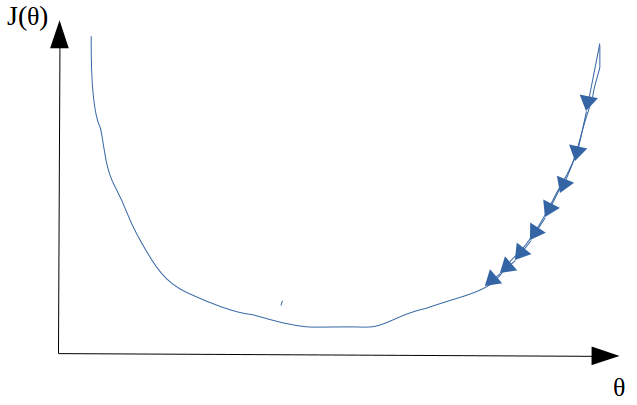
\includegraphics[scale=0.3]{slow_convergence}
    \caption{Small learning rate: slow convergence.}
  \end{minipage}
  \hfill
  \begin{minipage}[h]{0.45\textwidth}
    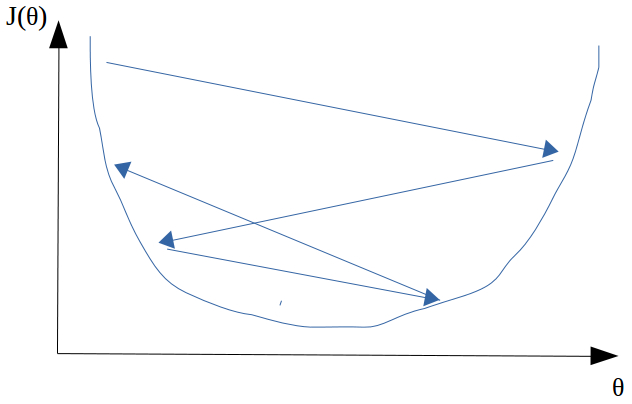
\includegraphics[scale=0.3]{divergence}
    \caption{Large learning rate: divergence.}
  \end{minipage}
  \caption{Intuitions behind tuning the learning rate on a convex cost function output.}
  \label{learning-rates-examples}
\end{figure}

However we know from \cite{yao-1999} ``J. D. Schaffer et al. \cite{schaffer-1990} have presented an experiment which showed that an ANN designed by the evolutionnary approach had better generalization ability than one trained by BP using a human-designed architecture''. Indeed, it is now known that the adaptive properties of GAs makes them an interesting choice to consider when designing an optimization solution.
\\
\\
The main architecture-design techniques that have so far been adopted to optimize an ANN are Simulated Annealing, Tabu search and Genetic Algorithms \cite{tereza-2006}.
\\
\\
As found in \cite{zhang-2000} and \cite{waghulde-2014} it is also known that ANNs are a promising alternative to various conventional classification techniques. As long as we have enough data to finely tune the weights and topology of an ANN on a representative set of data, the model should have relatively good generalization capabilities.

\section{Note on Neural Network Ensembles}

In order to obtain a Neural Network Ensemble, each ANN in the population makes a prediction for each example (positive or negative vote), then, for each example, the obtained majority of votes defines the prediction of the ensemble. In this project, the adopted elective scheme is one where the influence of each ANN during the election depends on its fitness. A fit ANN will influence the vote more than an weak individual. The weight of each vote is linearly decreasing from the fittest to the unfittest.

\chapter{Methodology and Design}

\section{Implementation Options}

The neural network implementation is the logic on which the experimentation is built, it is important to adopt a \textit{flexible} representation. In order to build a neural network able to adopt any topology two elements are required: an ANN representation (data-structure) and a corresponding \textit{forward propagation} method that fits this representation (see example \ref{forward-prop-example}).
\\
\\
Neural Networks have mostly been implemented either in Oriented Object, meaning that a Network, a Layer, a Neuron and a Synapse are each represented by their respective class definition. Another implementation design is inspired by scientist and mathematician programmers whom simply compute the mathematical behaviour of Neural networks, free from unnecessary abstractions. In this last one \textit{weights} and \textit{activations} are represented as Matrices and Linear Algebra is used to train and compute the output of the net.
\\
\\
Inspired by \cite{coursera-machine-learning-stanford}, I used matrices to represent the weight matrices and neuron activations. The forward method is then trivial to implement (see Listing \ref{listing:forward-propagation-code}). Using linear algebra also has the benefit of allowing us to alter its topology more easily than by manipulating neuron objects. Another key advantage of using this approach is the possibility to use a one-dimensional array to represent all the weights of the network by "flattening" the weight matrices. Doing so provides a real number encoded genotype that is ready to be used in the context of Evolutionary Algorithms.


\vspace{10pt}
\begin{lstlisting}[caption=Vectorized implementation of the forward propagation., label=listing:forward-propagation-code, captionpos=b]
mat NeuralNet::forward_propagate(mat X) {
    // return variable (output value of hypothesis)
    mat H;
    unsigned int total_nb_layers = get_topology().nb_hidden_layers + 2;
    vector<mat> Thetas = reshape_weights();
    vector<mat> Zs(total_nb_layers);
    vector<mat> As(total_nb_layers);
    unsigned int m = X.n_rows;
    // add bias unit
    mat bias = ones(m, 1);
    // feed input
    mat prev_activation = X;
    // forward propagate each layer
    for(unsigned int i=0; i < total_nb_layers-1 ; ++i) {
        // append bias
        As[i] = join_horiz(bias, prev_activation);
        // compute Z
        Zs[i+1] = As[i] * (Thetas[i]).t();
        // compute A
        prev_activation = sigmoid_matrix( Zs[i+1]);
    }
    // memorize predictions
    H = As[total_nb_layers-1] = prev_activation;
    return H;
}
\end{lstlisting}

The OO implementation has the benefit of providing a nice API to whatever software integrates with it. Such logic might feel like a natural way to solve this problem for a Java developer. However it is a less \textit{clean} implementation as it suggest incorporing many data-structures into our design which unnecessarily complexify the code. The OO approach also implies multiple nested for-loops to visit each node and four different abstractions to represent our stated elements. The Imperative Programming approach has the benefit of being computationaly faster because we can use an existing Linear Algebra library which makes best use of the CPU resources of the machine. Even though the mathematical approach requires to know the fundamentals of matrix computations, it has the benefit to be much easier to read since we can use vectorized operations. 

\section{Implementation Decisions}
In my implementation, I take the best of both worlds, I use Linear Algebra to compute the Neural Network behaviour which is all hidden in an Oriented Object API where you find the following Objects.

\begin{multicols}{3}
\begin{itemize}
  \setlength\itemsep{0.001em}
  \item NeuralNet
  \item Trainer 
  \item Evolutionary\_Trainer
 % \item Backpropagation\_trainer
  \item Net\_benchmark
  \item Data\_set
\end{itemize}
\end{multicols}


\section{Experimental Design}
The architecture of the application is represented by the \textit{Net\_Benchmark} class. This class allows to run different experiments based on the \textit{nature} of the initial population created the Genetic Algorithm. Each experiment produces a result file which can be visualised.
\\
\\
This course \cite{coursera-machine-learning-stanford} also bring to my attention that plotting the behaviour of my model is a key way to know how my learning algorithm is performing and avoid any ambiguity. This includes plotting the result of the error function over the number of iteration cycles (epochs) but also plotting the obtained network score as the parameters of the learning algorithm vary and else. I thrived to follow that thinking of consistently plotting the behaviour of my model in order to have multiple visual perspective of how my model and optimization algorithm is performing.


\subsection{Recorded Characteristics}
During each experiment, the key performance indicators listed below are evaluated and collected. From these results, the adequate plots are then generated using a simple Octave script.

\begin{multicols}{2}
  \begin{enumerate}
       \setlength\itemsep{0.0001em}
       \item  Number of epochs/generations
       \item  Mean squarred error
       \item  Prediction accuracy
       \item  F1 score (fitness)
       \item  Mean of scores of population
       \item  Median of scores of population
       \item  Variance of scores of population
       \item  Standard deviation of scores of population
       \item  Population size
       \item  Number of inputs 
       \item  Number of units per hidden layer
       \item  Number of outputs 
       \item  Averaged cross-validation score on 10 folds
       \item  Averaged cross-validation accuracy on 10 folds
  \end{enumerate}
\end{multicols}

\subsection{Data Set Segmentation}
The model is trained using the \textit{k-fold cross-validation} method. The training-set is used to optimize the weights and/or the topology of the model. The Validation and Training sets are used to evaluate the performances of the model when given . Separating the original data set in this way allow to evaluate how \textit{well} a model generalizes.
\\ \\
When cross-validating a model, the data set is iteratively separated into training and validation set in order to regularly train the model on \textit{new data} and therefore prevent overfitting. More details can be found in section \ref{section-the-overfitting-problem}.

\section{Neural Network Encoding}

Encoding neural networks, which is about finding the most adequate data representation to use as genotype has been widely investigated. Most existing methods fall into the following categories:
\begin{description}
  \setlength\itemsep{0.001em}
  \item[Binary Encoding scheme] \hfill \\
    The genotype contains a binary string of the weights of the neural network. Also called Conventional NeuroEvolution (CNE) \cite{schaffer-1990}, \cite{floreano-2008}, \cite{yao-1999}. Involves using a fixed topology.
  \item[Direct Encoding or Real Number Encoding scheme] \hfill \\
    The genotype contains a concatenation of all the parameters (weight, connections, etc.) of the network.
  \item[Indirect encoding scheme] \hfill \\
    The genotype contains only a description of the architecture.
  \item[Development Rule Represention scheme] \hfill \\ 
    The genotype contains the production rules that represent how the parameters can be produced. In Cellular Encoding (Gruau’s (1993) Cellular Encoding), the genotype is a program written in a specialized graph transformation language (as explained in stanley-2002)
  \item[Graph encoding scheme] \hfill \\
    The genotype contains a more explicit graph-structure in order to be able to use a GA and avoid the permutation problem (irrrelevant for fully connected ANNs).
\end{description}

\section{Fitness Function}
In order to use a Genetic Algorithm, we essentially need two things: a genetic representation of a single solution and a fitness function.The fitness function is there to return a numerical expression representing the quality of a solution.Typically contained between 0 and 1, the fitness function gives a mean to compare two individuals and know which one performs better on the task at hand, the best fitness function is problem specific. Because the fitness function represents the criterion by which a certain individual will be selected over an other, selecting the right one is an important matter. 

\subsubsection{Mean Squared Error}
The simplest and most well-known approach for a cost or a fitness function is the Mean Squared Error (MSE, see \ref{MSE}).

\begin{equation}
MSE = { 1 \over N } \sum_{i=1}^{m} (h_{\theta}(x_i) - y_i)^2
\label{MSE}
\end{equation}


\subsection{Fitness function for Imbalanced Data}
In Data Analysis, it is common to have to work with \textit{unbalanced data sets}, in such context the prediction accuracy of the model does not represent well its ability to make predictions of good quality. This is why more meaningful calculations taking into account notions like the \textit{precision} and the \textit{recall} of a model have been developed.

\subsubsection{Precision and Recall}
Both the precision and the recall of a model are based on the concepts of true/false positives/negatives (see in Table \ref{table:true_pos}). Considering such concepts in the score calculation is highly prefered than only using the prediction accuracy.

\begin{table}[h]
\centering
\begin{tabular}{|l|cc|}
  \hline
  \diagbox{Predicted output}{Actual output} & 1 & 0 \\
  \hline
  1   &   true positives   &  false positives    \\
  0   &   false negatives  &  true negatives     \\
  \hline
  \end{tabular}
  \caption{Concepts of true false positives negatives}
  \label{table:true_pos}
\end{table}

Essentially the intuition behind using more sophisticated variables to compute the score comes from the fact that good classifier is a classifier that has the following properties:
\begin{enumerate}
 \setlength\itemsep{0.001em}
 \item Many to all positives examples are classified as positive (true positives)
 \item Many to all negatives examples are classified as negative (true negatives)
 \item Very little to zero positives examples are classified as negative (false negatives)
 \item Very little to zero negatives examples are classified as positive (false positives)
\end{enumerate}


\subsection{F1 score}
The F1 score makes use of these concepts of precision and recall to provide a single-numbered indication of how good the model is at accurately predicting positive when it should do so and negative correspondingly. 
\\ \\
In the implementation, this value is scaled between 0 and 100 to be able to visualise it alongside the accuracy. A higher scale fitness function also has the advantage of being a more precise comparison value since values between 0 and 1 can only be compared up to so many decimal places.

\begin{equation}
precision = { \text{TP} \over (\text{TP}  + \text{FP} )} , recall = { \text{TP} \over (\text{TP}  +  \text{FN} )}
\end{equation}

\begin{equation}
F_{1} score = { \text{precision} \times \text{recall} \over (\text{precision}  +  \text{recall} )}
\end{equation}

\subsection{Matthews correlation coefficient}
% More details here: https://en.wikipedia.org/wiki/Matthews_correlation_coefficient
The F1 score function in itself is a meaningful enough score calculation for many problems, however it does not take into considerations the true negatives. The Matthews Correlation Coefficient is therefore an even more \textit{complete} measure. 
\begin{equation}
MCC = { \text{TP} \times \text{TN} - \text{FP} \times \text{FN} \over \sqrt{ (\text{TP} + \text{FP}) (\text{TP} + \text{FN}) (\text{TN} + \text{FP}) (\text{TN} + \text{FN})  } }
\end{equation}


\subsection{The Crossover Problem}

Because of the functional nature of ANN's (forward propagating using a set of coefficients) it is understandable that it is only the rightness of the combination of coefficient that represent its ability to predict well. Therefore, by swaping a subset of the coefficient with a foreign subset, one cannot assume that a better offspring will be produced. Given two high-performing ANN's mating them often leads to a loss of prediction ability. Throughout this experiment, it was observed that applying a traditional GA with a crossover operation only produced bad offspring (a.k.a \textit{destructive} crossover).
\\
\\
This leads us to Evolutionary Programming, a subfield of evolutionary computation where there is a strong tendency to minimize the crossover operation to impacting a much smaller percentage of the genotype (Differential Evolution, Evolution Strategies etc.) or not performing any crossover operation at all (nonmating).

\subsection{Encoding decisions}
Because of the goals of neuroevolution methods, the known issues with binary-encoding (see quote \ref{quote-yao-binary-encoding}) and the scope of this project, a choice was made to use a Real Number encoding. Two main direct encoding strategies have been used so far. The first one isolates the evolution of the architecture from the evolution of the weights whereas the second evolves both simultaneously. In this project the second approach is used (see model used for chromosomes \ref{table:genome-encoding} and example \ref{table:genome-encoding-example}).

\begin{table}[h]
\centering
\begin{tabular}{| l | p{5cm} |}
  \hline
    topology    &  weights  \\
  \hline
  \end{tabular}
  \caption{model used for chromosomes: Direct encoding. (One dimensional array containing a topology description followed by the flattened weight matrices).}
  \label{table:genome-encoding}
\end{table}

\begin{table}[h]
\centering
\begin{tabular}{|l|l|l|l|l|l|l|l|l|l|l|l|l|l|l|l|}
  \hline
   5 & 1 & 0.21 & -0.92 & 0.22 & 0.71 & -0.15 & \dots & -0.99 & -0.83 & 0.5 & 0.32 & -0.1 & 0.89 & 0.65 \\
  \hline
  \end{tabular}
  \caption{Example Real Number encoding (5 hidden units, 1 hidden layer).}
  \label{table:genome-encoding-example}
\end{table}

\begin{quotation}
"The canonical genetic algorithm (GA) [13], [14] has always used binary strings to encode alternative solutions, often termed chromosomes. Some of the early work in evolving ANN connection weights followed this approach [\dots] However, a tradeoff between representation precision and the length of chromosome often has to be made. If too few bits are used to represent each connection weight, training might fail because some combinations of realvalued connection weights cannot be approximated with sufficient accuracy by discrete values. On the other hand, if too many bits are used, chromosomes representing large ANN’s will become extremely long." Yao et al.\cite{yao-1999}
\label{quote-yao-binary-encoding}
\end{quotation}

From an engineering perspective, using real valued vectors to represent individuals also has the following advantages:

\begin{itemize}
  \setlength\itemsep{0.001em}
  \item Shorter genomes will be manipulated. \\ 
    (This is especially interesting for Deep Belief Networks)
  \item It is a simpler and leaner solution to implement and therefore build upon
\end{itemize}

In TWEANN (Topology and Weight Evolution of Artificial Neural Networks), NEAT-like methods\cite{stanley-2002} imply using a graph algorithm to represent ANN's instead of using a fully connected ANN with enough hidden layers and hidden units. A solid argument for using such method is that NEAT methods are more autonomous. When using a traditional ANN, the developer has to find the best topology as well by himself. When using a GANN, the developer still has to insert a valid \textit{largest possible topology}. However when using NEAT, there is no need for the developer to provide a large enough topology because the topology gets larger by adequately adding nodes to the graph.

\section{The Overfitting Problem}
\label{section-the-overfitting-problem}

When optimizing the parameters of an ANN, the aim isn't to build a predictive model only able to work on the given data set but "to to build a statistical model of the process which generates the data"\cite{bishop-1995}. In other words, we want to find the model that replicates the behaviour of the pattern held by the data set in order to use it for predictions that will also work on new data. We are interested in training a model with a \textit{high generalization capability}. Since overfitting is a common problem, there are multiple known ways to deal with it. This section discusses the \textit{Cross-Validation} and the \textit{Regularization} techniques.

\subsection{Neural Network k-fold Cross-Validation}
In order to find a model with high generalization capabilities, we will want to make sure that the complexity of the model is appropriate. An overly simple model class will tend to \textit{underfit} (also referred to as high bias), whereas an overly complex model class will tend to \textit{overfit} (also referred as high variance). The process of finding the right fit for the data at hand is sometimes referred to as the \textit{Bias-Variance tradeoff}. This situation is well summarized by the Figure \ref{bias-variance-tradeoff}.
\\ \\
For example, if we were to use a regression model class, we would have to find the adequate number of polynomials to use. As you can imagine, a single polynomial (linear regression) will only be able to fit linear patterns. If the pattern is more complex (of higher degree) then we shall use a higher order polynomial (the one with just enough degrees of freedom). However, in the context of neural networks. With Neural Networks, the complexity of the model is based on the number of the hidden units per layer and the number of hidden layers.

\begin{figure}[!h]
  \begin{center}
    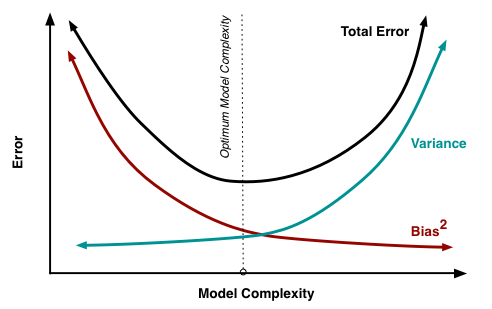
\includegraphics[scale=0.65]{biasvariance_fortmann_roe}
  \end{center}
  \caption{Bias and Variance contributing to total error. Source: Scott Fortmann Roe\cite{fortmann-2012}}
  \label{bias-variance-tradeoff}
\end{figure}

In order to simulate feeding new data to our model, the data set is divided into \textit{k} \textit{folds} (or subsets). In our case, we use the default value of $k = 10$, we are doing a 10-fold cross-validation. Once done, a single subset will be used as test set (also referred as \textit{cross-validation} set) while all other subsets are used as training data. This process can be illustrated by the Figure \ref{figure-cross-validation}. The plots presented in the result section show a single run of the 10 fold cross validated optimization algorithm, within a total number of generations, the model is trained on a different validation fold (which explains why the score sometimes drop).

\subsubsection{Maintaining the positive/negative example ratio}

Because most data-sets are more or less \textit{skewed}, simply using cross-validation isn't enough to train the network in an elegant manner. Preserving the imbalance ratio within each validation fold ensures that there will be no case of optimization over a subset of positive examples only. In other words, each fold must be as \textit{representative} as possible. Without doing so, a probability of a \textit{biased training} is introduced for each validation fold used during training.

\begin{figure}[!h]
  \begin{center}
    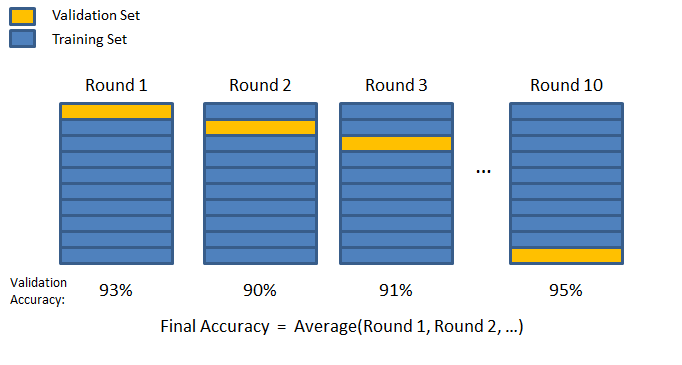
\includegraphics[scale=0.75]{cross_validation_mccormick}
  \end{center}
  \caption{Illustration of the 10 fold cross-validation method. Source Chris Mccormick\cite{mccormick-2013}}
  \label{figure-cross-validation}
\end{figure}

\subsection{Neural Network Regularization}
Regularization is a well-known method to prevent the common problem of overfitting. We know from \cite{yao-1999} that "The evolutionary approach also makes it easier to generate ANN’s with some special characteristics. For example, the ANN’s complexity can be decreased and its generalization increased by including a complexity (regularization) term in the fitness function". Using regularization, the error function is expressed as follows (see \ref{error-function-model}) where $\Omega$ is known as the regularizer. This method wasn't used in the current experiment but must be stated for better completeness.

\begin{equation}\label{error-function-model}
  J = E + \Lambda\Omega
\end{equation}

\cite{yaochu-2004} popular approach for regularizing ANNs is the \textit{weight decay} (see \ref{weight-decay})
\begin{equation}\label{weight-decay}
  \Omega = {1 \over 2} \sum_{i}^{} \theta_{i}^{2} \text{,where i is the index summing all the weights}
\end{equation}

\section{The Competing Conventions Problem}

Also known as the Permutation Problem, the Competing Conventions problem describes the phenomenon of having two or more neural networks with different permutations of weights but identical predictions. In other words, many individuals in the search space correspond to the same solution. As for the NEAT method \cite{stanley-2002}, the co-evolution of topology and weights of ANNs tackles a wider problem. Due to the co-existence of various topologies in the same population, the problem that arises is how to crossover ANNs with genomes of different length?
\\ \\
The proposed solution initially instantiates neural networks with random weight and topologies (represented as chromosomes: a vector a real numbers). However, the limit of the search space of this algorithm is the length of the vector encoding the neural network, therefore, a \textit{maximal topology} must be given before training. Note that this mean that it would be interesting to search for a more dynamic approach comparable to NEAT \cite{stanley-2002} to break down this limit and search through the entire search space. 
\\ \\
In order to compare neural networks of diverse topologies, this solution uses DE to apply a \textit{mutative crossover} for each element of the genome up to its corresponding last weight. The last weight is found after having applied the mutative crossover(or not) on the hyper-parameters by calculating the total number of weights of the network depending on these values. The rest of the vector is ignored and will not be used unless a later mutative crossover results in the elements of the vector corresponding to the \textit{Number of Hidden Layers} or \textit{Number of Hidden Units per Hidden Layer} to be greater. This is how as the Evolutionary Optimization continues, the entire population explores and converges towards a distinct topology. 
\\ \\
The problem that emerges from this is the existence of different topologies with different weights performing the same predictions. This sometimes causes the algorithm to have multiple networks with identical performances but different topologies being the fittest individuals. There is no straight answer for which network is best keeping, however both contain an interesting information. The two main ingredients to paliate to this problem is 1) forcing a mutative-crossover between the two best networks and 2) Using cross-validation will sometimes get rid of the competing networks as some of them will not perform well on the new data.


\section{Data Preprocessing}

It is common in the field of Machine Learning to need to preprocess data sets \cite{coursera-machine-learning-stanford}, for example to make sure that all used features are on a similar scale. Since ANNs multiply weights and inputs, then sum the results and finally outputs it, it is understandable that if a one attribute is of much larger scale than the others, this attribute will have a greater influence on produced output. \textit{Data standardization} removes this problem, all features have about the same influence over the prediction. Ultimately, it allows optimization methods to converge more quickly because weights are only used to map the pattern of the data set and not too counter-balance the existence of out-of-scale attributes.

\subsection{Feature Scaling}
I learned from \cite{coursera-machine-learning-stanford} \textit{Feature scaling} is used to get all feature values into a $-1< x_i < 1$ range, this also perfectly matches the range of the weights. In order to transform features into their corresponding scaled values, we use a technique called \textit{Mean normalization}. Mean-normalization is used to make features have approximately zero mean (see Formula \eqref{mean-norm-formula}).

\begin{figure}[h]
  \begin{equation}
  x_i \gets {x_i -\mu \over max - min} \text{, where $\mu$ is the average value of $x_{i}$}
  \end{equation}
  \caption{Mean-normalization formula}
  \label{mean-norm-formula}
\end{figure}

\section{Selection of Control Variables of DE}

Some basic rules have been identified as reasonnable choices for DE's control variables \cite{storn-1997}, the Crossover Rate (CR) and the Differential weight F. A high CR will speed-up convergence. Effective values of F are contained within 0.4 and 1, values outside this range have been observed as only occasionally effective.


\chapter{Results}

This chapter presents the results obtain of using DE with the mutation schemes described in \ref{equations:mutation-schemes} as well as using PSO. The size of the genome was limited by the maximum topology: 2 hidden layers, 20 hidden units. A training sequence as shown in Figure \ref{malignant-perfs} is composed of a number of a given number of generations. 
\\ \\
In order to train a model that will generate well on new data, the 10 fold cross validation method is used. In this total number of generations the algorithm uses different validation set one after the other. If a total of 1650 generations was given, the optimization algorithm will spend 150 generations using a different validation fold (10 folds + 1 final run on entire set, $1650/11=150\text{generations per fold}$). This process explains why sudden drop and rise can be seen as it shows the current best neural network not as good at making predictions on new data.
\\ \\
As previously stated, three data-sets were used in this experiment, for each problem, three main plots are produced.
\begin{description}
  \setlength\itemsep{0.001em}
  \item [General performance plots] \hfill \\
  Average F1 score and prediction accuracy among replicates as the optimization is performed.
  \item [Mean of the fitness values] \hfill \\
  Among all the individuals, in order to observe the pace at which the population improves.
  \item [Variance of the fitness values] \hfill \\
  Among all the individuals, in order to evaluate divergence/convergence phases.
\end{description}
For the sake of clarity and presentation, each one of these plots will not be commented as it would involve unnecessary repetitions. However, the plots obtained on the \textit{recurrence} and the \textit{survival} problem can be found in appendices \ref{complementary-results-recurrence} and \ref{complementary-results-haberman} respectively.

\newpage

\section{Breast Cancer: Malignant or Benign?}

\subsection{Differential Evolution (mutation scheme: DE/RAND)}

As Figure \ref{malignant-perfs-DE-rand} shows, the EA does not behave smoothly as you would expect from a training algorithm like BP. Note that the fitness function used is the F1 score. I observe that DE trains a neural network with near state-of-the-art performances \ref{table:state-of-the-art-comparison} (94.7\% F1 score $\approx$ 95.5\% accuracy). Amongst the 16 replicates, the most suitable model was found with 9 hidden units and 1 hidden layer. The error bars show that by the $700^{th}$ generation DE will have found a model with a score and accuracy around 93\% depending on the fold being used.

\begin{figure}[h]
  \centering
  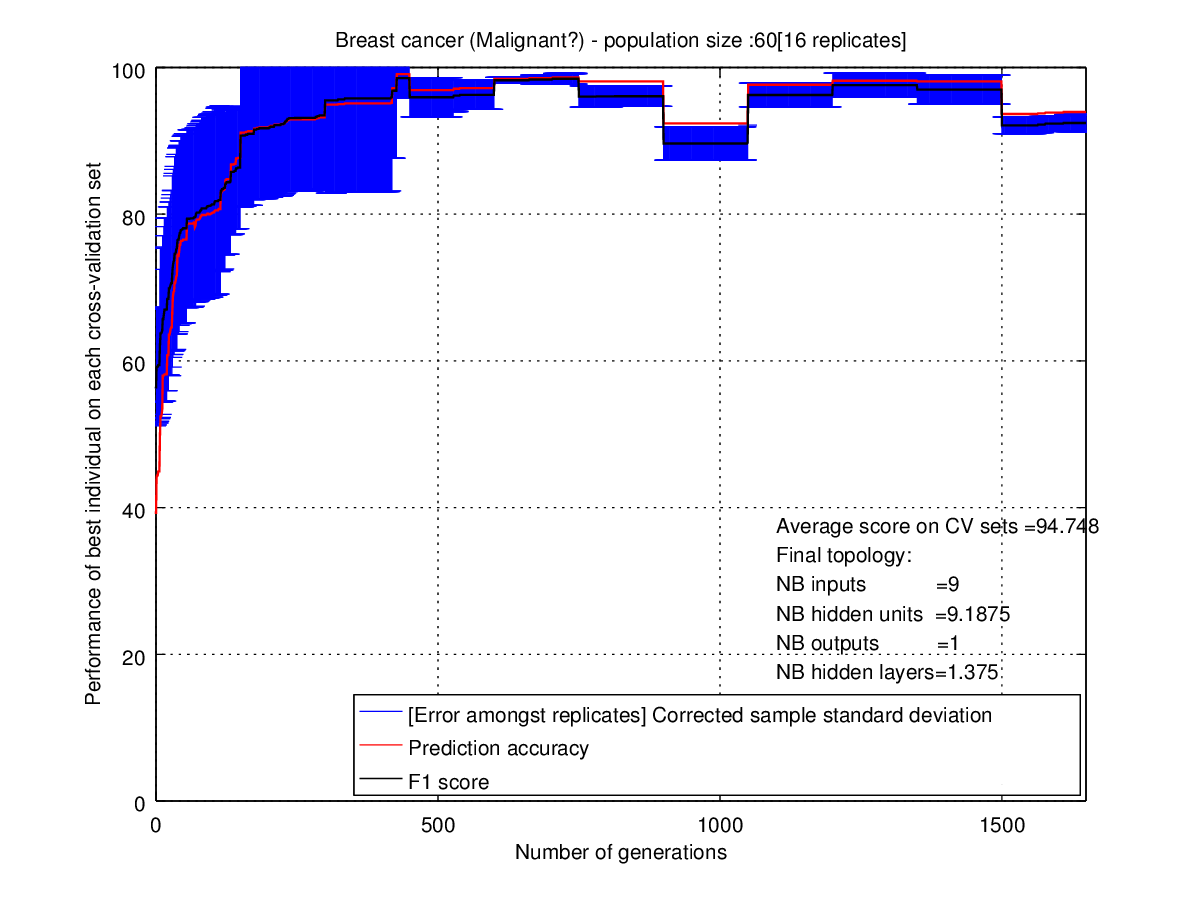
\includegraphics[scale=0.7]{malignant-performancesVSepochs-DE}
  \vspace{-12pt}
  \caption{Optimization of the neural network population (DE-rand)}
  \label{malignant-perfs-DE-rand}
\end{figure}

The Figure \ref{malignant-mean-DE-rand} shows how the overall population gets fitter as the model is trained, as you would expect with any EA. The \textit{exploration} and \textit{convergence} of DE can be explained from the figures \ref{malignant-perfs-DE-rand}, \ref{malignant-mean-DE-rand} but primarily \ref{malignant-variance-DE-rand}. Figure \ref{malignant-variance-DE-rand} shows that by the $1000^{th}$ generation, the entire population will have reached a highly similar fitness. Looking at the slopes of the curves in figures \ref{malignant-perfs-DE-rand} and \ref{malignant-mean-DE-rand} it is observed that they both have reached a \textit{plateau}, this confirms that the probability that DE produces better offspring is drastically reduced.
\\ \\
For this experiment, a \textit{direct} termination criteria was used: 150 generation per fold ($150\times11=1650$ generations). When using a \textit{derived} termination criteria such as comparing the variance value with a limit $\epsilon$ amongst multiple replicates, the separation of cross-validation folds can be noticed when the slope is abruptly negative (see "step" effect on Figure \ref{malignant-perfs-DE-rand} or \ref{malignant-mean-DE-rand}, as the amount of generations per fold increases, this phenomenon tends to be less present). 

\paragraph{Exploration and exploitation}
Also, the two phases of population-based optimization can be noticed: \textit{exploration} (or \textit{divergence}) and \textit{exploitation} (or convergence) in Figure \ref{malignant-variance-DE-rand}. Initially, the variance of the fitness values of the individuals steadily gets higher. The difference between the fittest individual and the unfittest gets higher, in other words, the EA consistently finds better individuals. The first phase demonstrates a clear gap between the worst and the fittest individuals, as the EA keeps mating and mutating, better individuals are found, \textit{the EA is exploring}. However, around the $1000^{th}$ generation, for some reason, the EA struggles to find better solutions, it reaches a plateau where the fittest individuals finds no stronger contestant. However, the EA still mates and mutates the best individuals which produce offsprings that are fitter than the worst individuals of the population, therefore, the fitness gap between the worst individuals and the fittest gets smaller and smaller: \textit{the EA has converged}. This phenomenon can be observed on each data set and for PSO as well.

\begin{figure}[h]
  \centering
  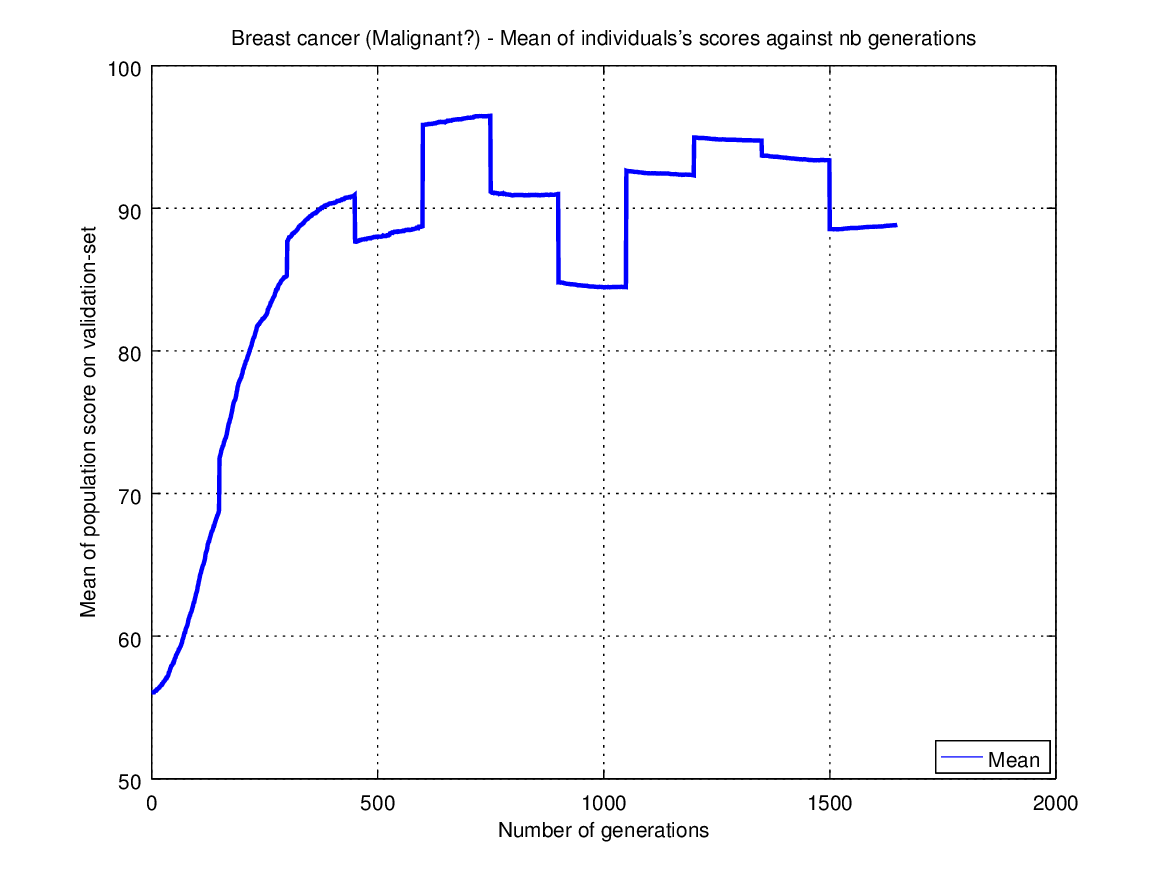
\includegraphics[scale=0.7]{malignant-meanVSepochs-DE}
  \vspace{-12pt}
  \caption{Overall population gets fitter (Mean, DE-rand)}
  \label{malignant-mean-DE-rand}
\end{figure}

\begin{figure}[h]
  \centering
  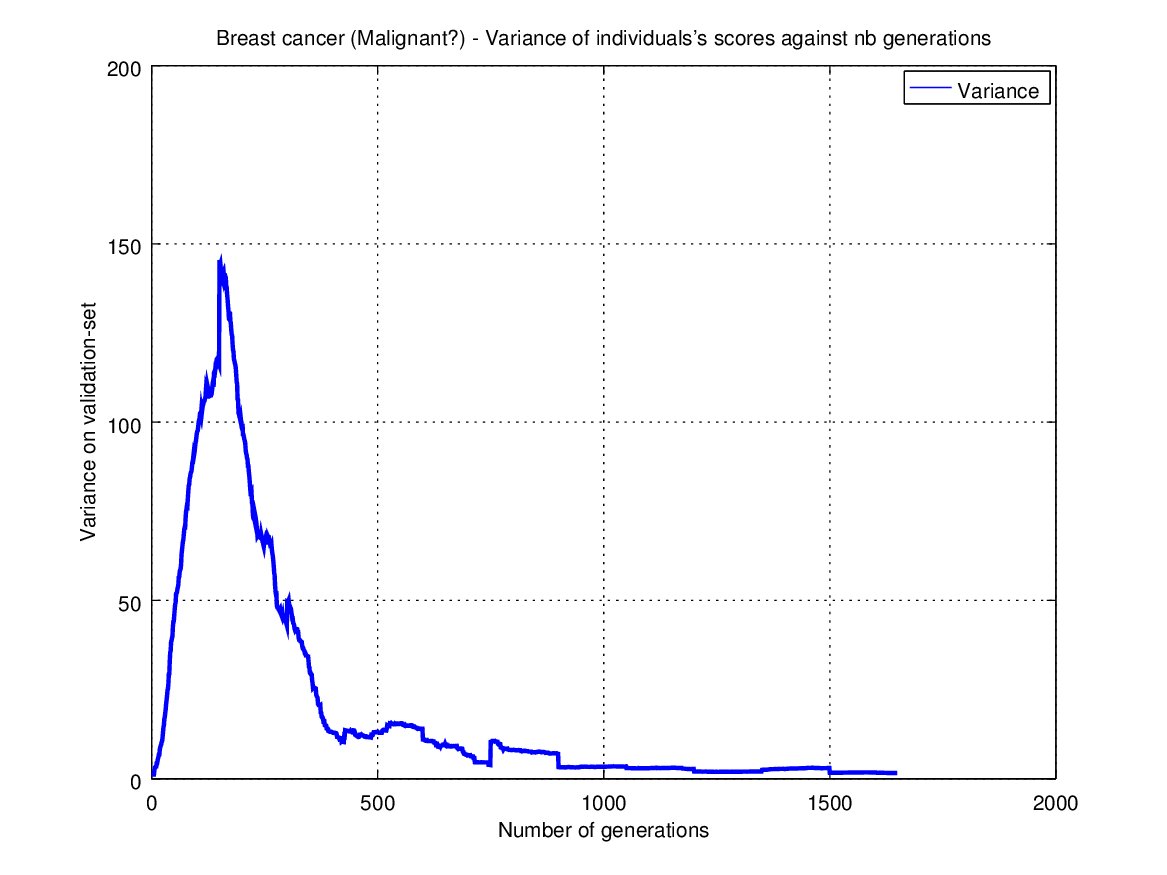
\includegraphics[scale=0.7]{malignant-varianceVSepochs-DE}
  \vspace{-12pt}
  \caption{Convergence towards optimal solution (DE-rand)}
  \label{malignant-variance-DE-rand}
\end{figure}


\begin{figure}[h]
  \centering
  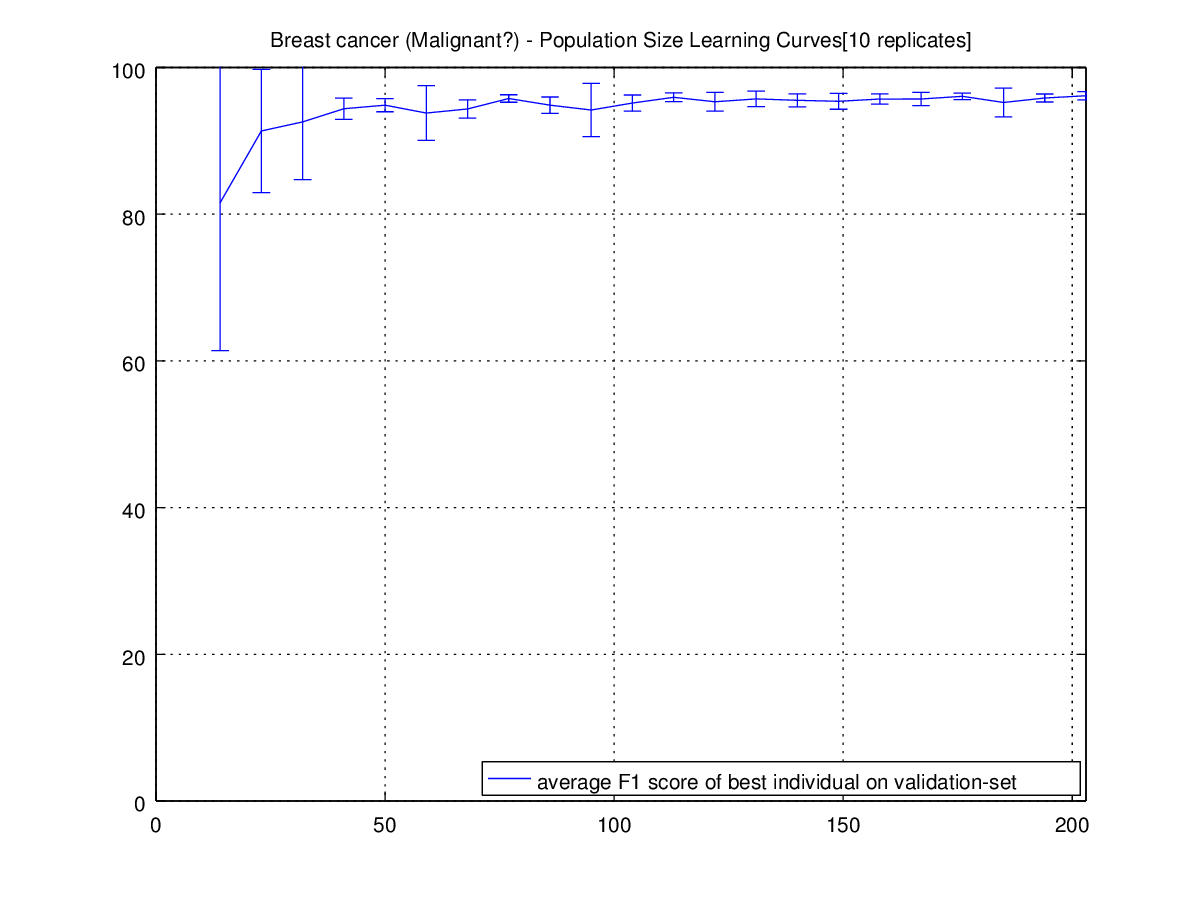
\includegraphics[scale=0.95]{malignant-learning_curve_pop_size-DE}
  \vspace{-12pt}
  \caption{Average population fitness on increasingly large populations (DE-rand)}
  \label{malignant-increasing-pop-size}
\end{figure}

The Figure \ref{malignant-increasing-pop-size} illustrates the quality of the trained neural networks with larger and larger population size. It is observed that on average using a population size superior to 60 individuals does not help in optimizing the model any more.

\clearpage

\subsection{Differential Evolution (mutation scheme: DE/BEST)}

\begin{figure}[h]
  \centering
  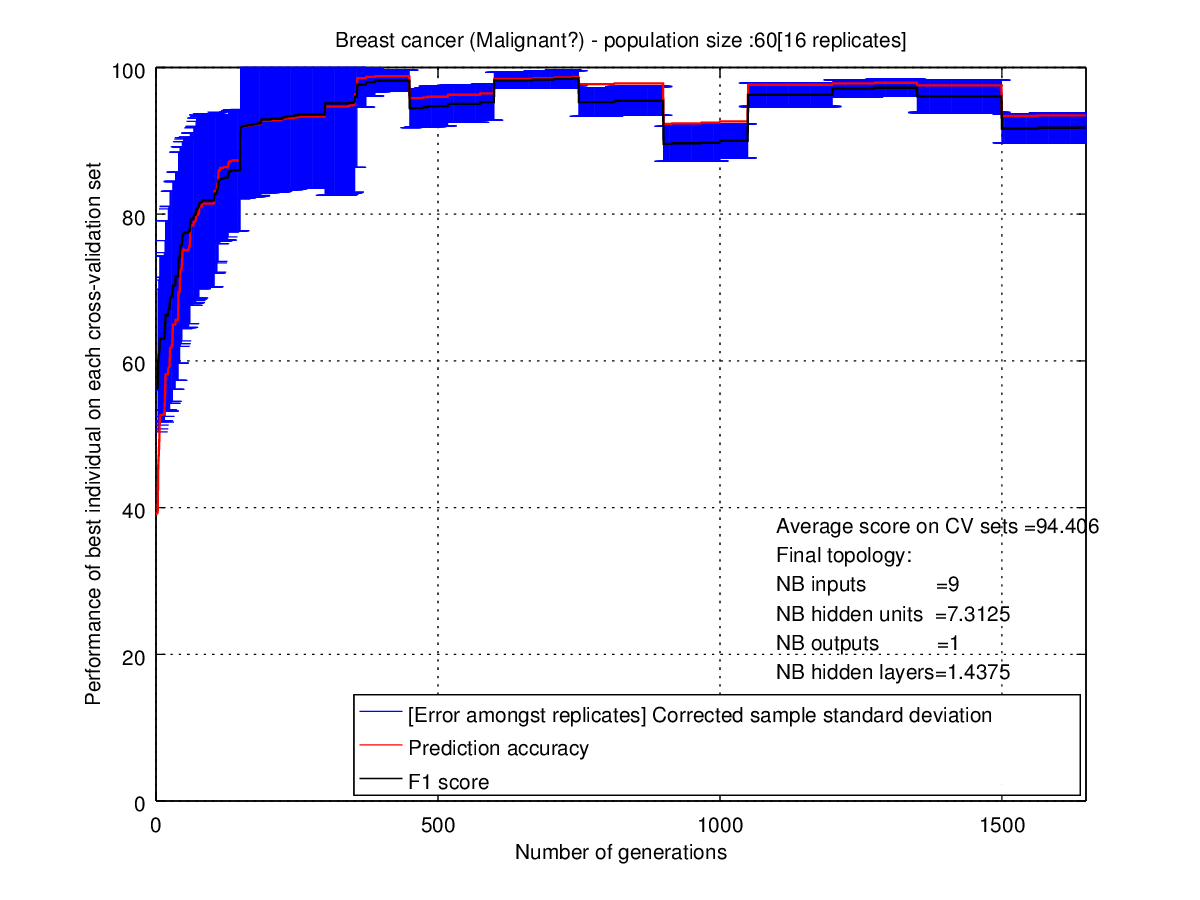
\includegraphics[scale=0.7]{malignant-performancesVSepochs-DE-BEST}
  \vspace{-12pt}
  \caption{Optimization of the neural network population (DE-best)}
  \label{malignant-perfs-DE-best}
\end{figure}

\begin{figure}[h]
  \centering
  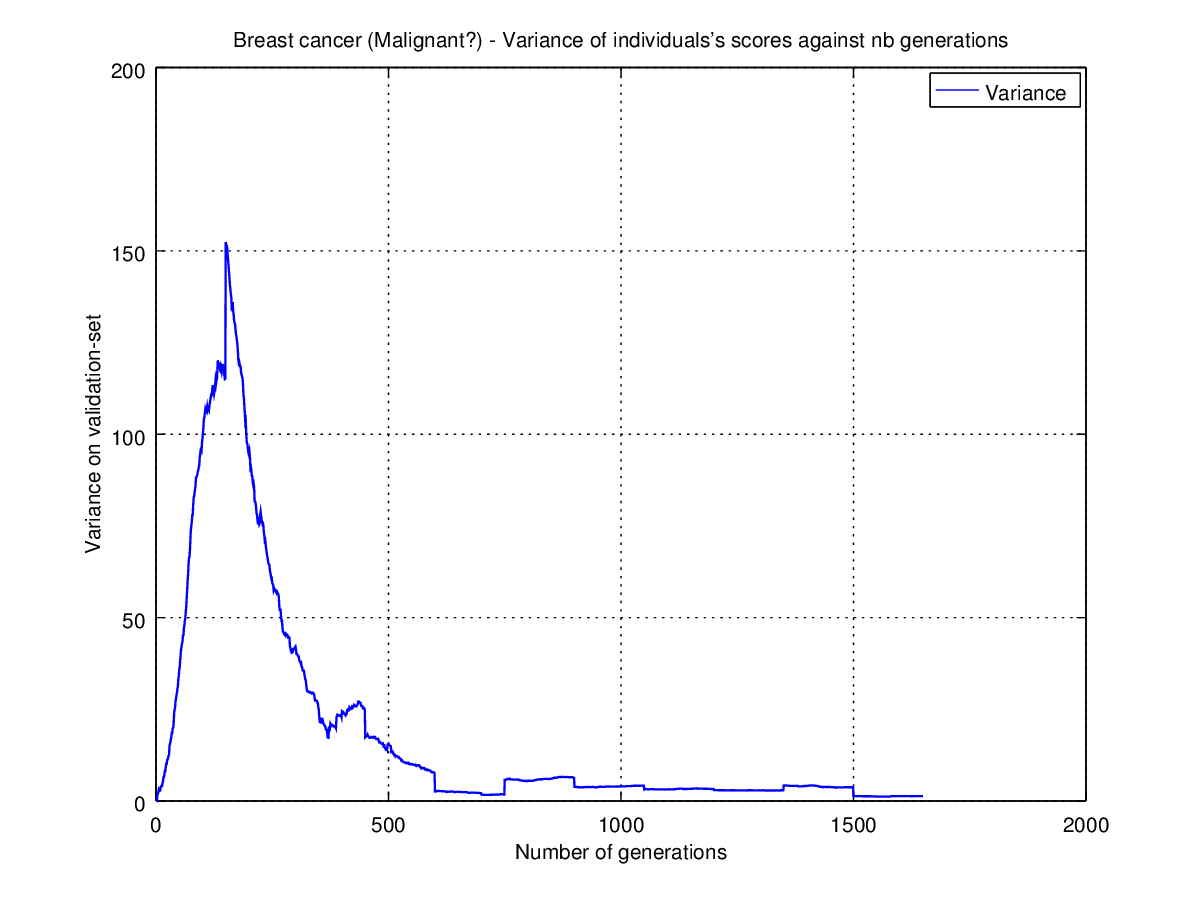
\includegraphics[scale=0.7]{malignant-varianceVSepochs-DE-BEST}
  \vspace{-12pt}
  \caption{Convergence towards optimal solution (DE-best)}
  \label{malignant-variance-DE-best}
\end{figure}

Globally, the algorithm behaves almost identicaly to the random mutation scheme version. The EA \textit{explores} and \textit{exploits} at relatively the same periods and with about the same slope. 
\\ \\
I note that the algorithm finds a smaller topology (7 hidden neurons per layer against 9 for DE-Rand) while obtaining a neural network with similar prediction ability of 96\%. The variance decreases following the same pattern which ressembles a noisy $e^{-x}$.  

\subsection{Particle Swarm Optimization}


PSO shows an ability to get very fast good results, it can be noticed by looking at how abruptly the training algorithm initially optimizes the neural network. In less than 100 generations, the algorithm converges towards a solution when it took on average $\approx500$ generations to DE to obtain a model with an accuracy near 95\%. 
\\ \\
The \textit{exploitation} capability of PSO is therefore much greater than DE's. However, this comes with the limit that PSO tend to easily fall into a local optima or prematurely converge as it is the case here. In order to prevent such problem, one must make sure that the population maintains a certain degree of \textit{diversity}. Picking an appropriate scaling factor for the velocity at which particles move around the search space. If this isn't done, the swarm will have converged towards the same solution and no optimization will then be possible.
\\ \\
Since the swarm  prematurely converges towards a non-optimal solution, I note that in essence, PSO is more efficient for local searches than it is for global ones.

\begin{figure}[h]
  \centering
  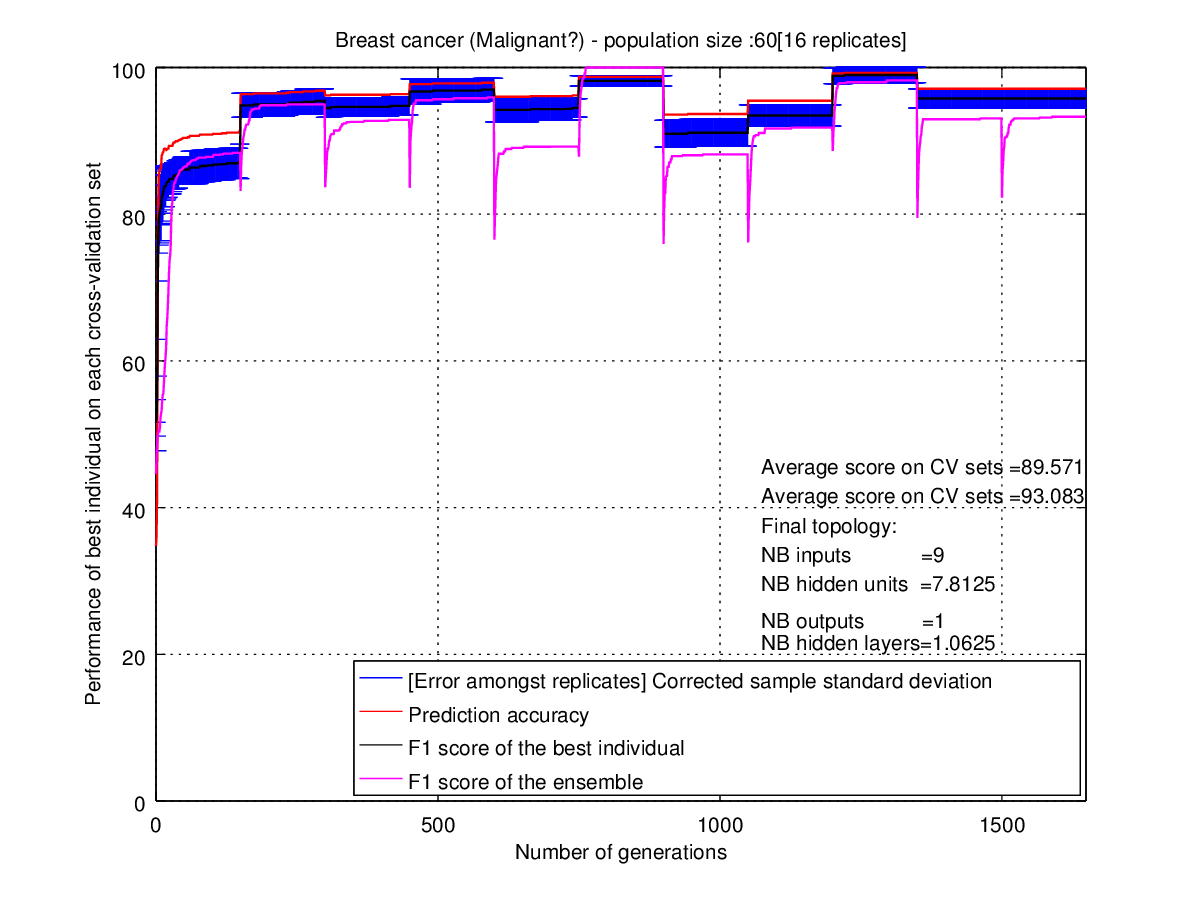
\includegraphics[scale=0.7]{malignant-performancesVSepochs-PSO}
  \vspace{-12pt}
  \caption{Optimization of the neural network population (PSO)}
  \label{malignant-perfs-PSO}
\end{figure}

\begin{figure}[h]
  \centering
  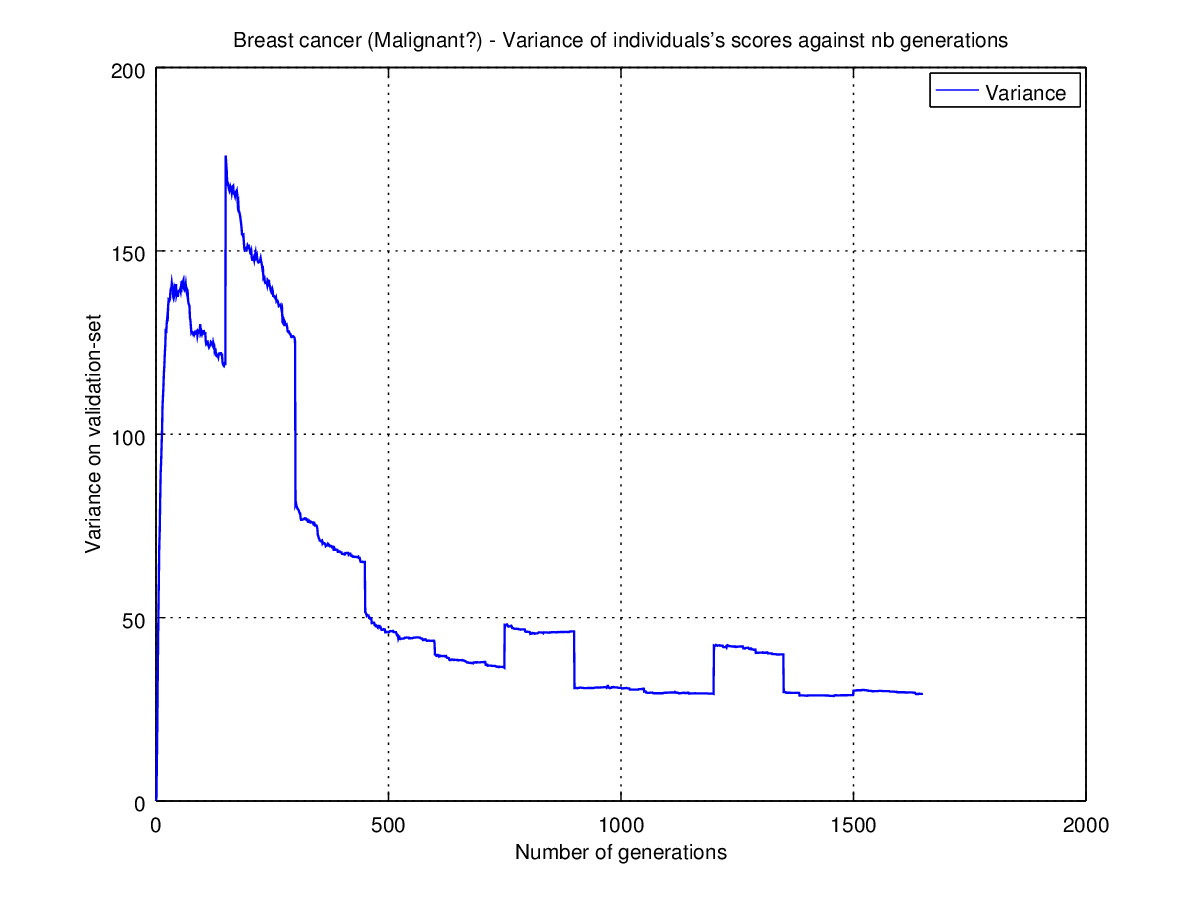
\includegraphics[scale=0.7]{malignant-varianceVSepochs-PSO}
  \vspace{-12pt}
  \caption{Convergence towards sub-optimal solution (PSO)}
  \label{malignant-variance-PSO}
\end{figure}

\begin{figure}[h]
  \centering
  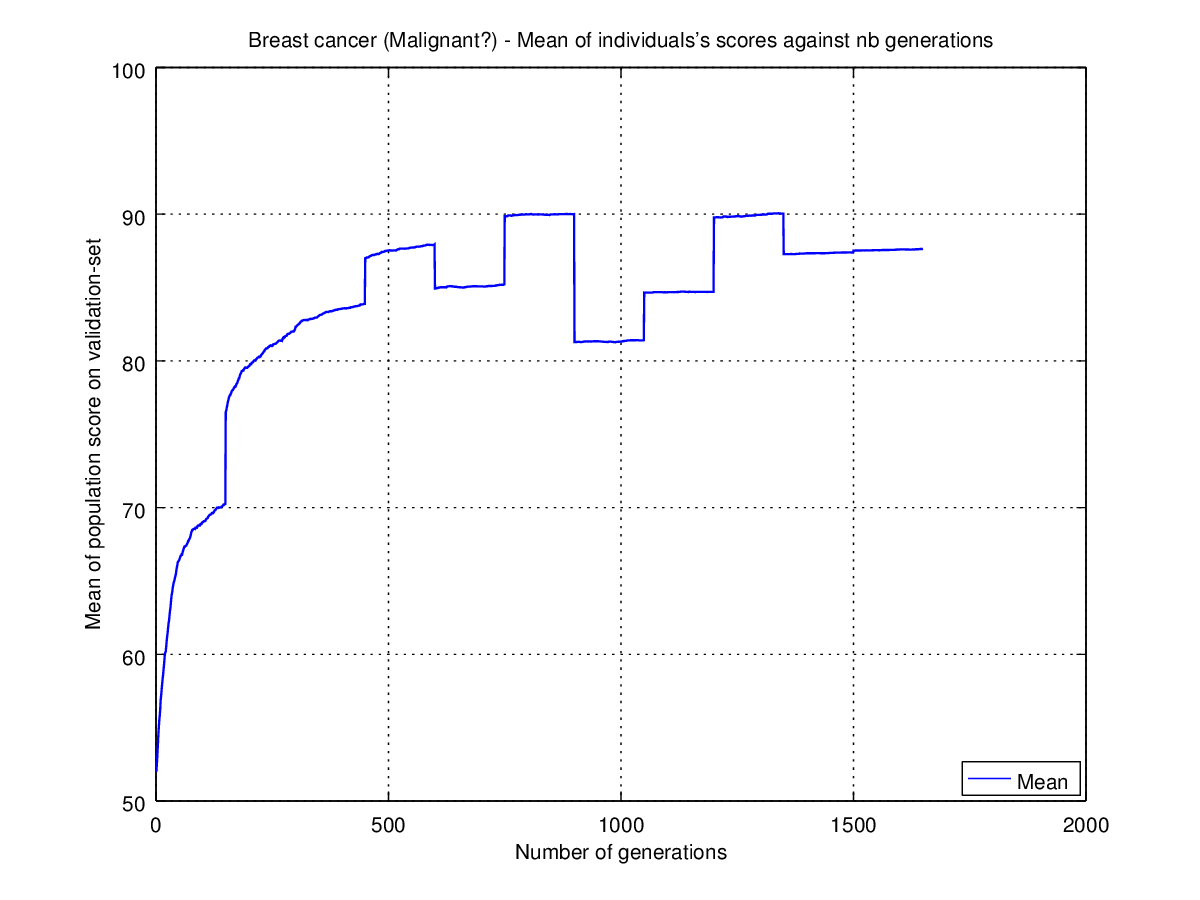
\includegraphics[scale=0.7]{malignant-meanVSepochs-PSO}
  \vspace{-12pt}
  \caption{Overall population gets fitter (Mean, PSO)}
  \label{malignant-mean-PSO}
\end{figure}

\clearpage

\section{Breast Cancer Recurrence}

The results in Appendix \ref{complementary-results-recurrence} DE optimizes the model relatively well and in a very stable fashion. Although this problem requires a longer training, the curve reaches the top of the graph in less than 500 generations. The error bars show that the best neural network of the population tends to have an F1 score between 80 and 100. Previous experiment showed that this wasn't possible with only 1500 generations. I observed that what happen is that not enough generation per layer was given for the algorithm to be able to learn from the current validation fold. 

\section{Haberman's survival}

From the results in Appendix \ref{complementary-results-haberman} it is quickly visible that generating a model able to predict the likelyhood of a patient to survive the surgery for breast cancer within 5 years is probably the most difficult problem of the three studied here. Both DE and PSO generate at best an ANN with a score $\approx60\%$ which is equivalent to $\approx70\%$acc. However, the error bars of show a standard error of the individual's f1 score among replicates is superior to 10 indicating that the population is still diverse and therefore the algorithm has not yet converged towards a global optima.
  
\section{Using a Derived Termination Criteria}

This section presents the behaviour of DE when using a \textit{derived} termination criteria based on the variance of the fitness values of the population. Here, the training on the current validation fold is stopped (and followed by the training on the next fold) whenever the variance is inferior to $\epsilon$, $\epsilon$ being equal to the value of variance at its highest divided by 20. Appreciate that the value 20 was chosen arbitrarily, it is unlikely that it would work on all problems. Typically $\epsilon$ would be set to a value such as $10^{-n}$. However, what is important is that $\epsilon$ is based on the current problem, which is why the decision of using the height of the variance peak is justified.
\\ \\
The first observable pattern is how much \textit{smoother} the training curve is. Precisely, the cross-validation phases that were distinclty separated by a number of 150 generations in Figure \ref{malignant-perfs-PSO} now tend to disappear. It can also be observed within the course of a 1000 generations, the algorithm trains an ANN with an average of 95.446\% accuracy accross all validation sets when the initial run of DE was forced to finish its 1650 iterations (see \ref{malignant-perfs-DE-rand}).
\\ \\
This \textit{derived} termination criteria demonstrates here the advantage of making the search $\approx \frac{1}{4}^{th}$ faster. In essence the search could be made even faster, however since the cross validation method is used, a fairness between fold must be maintained in order to prevent introducing a learning bias. Therefore, the algorithm is forced to attempt finding better solutions during the first third of the total number of generations for the current fold. In the same way that the value of \textit{10} is arbitrary in the 10-fold cross validation method, this one was selected by means of empirical study. 
\\ \\
This method also demonstrates a better ability at training the ensemble without overfitting. By the end of the training, the obtained ANN ensemble appears to be about as accurate as the best individual.

\begin{figure}[h]
  \centering
  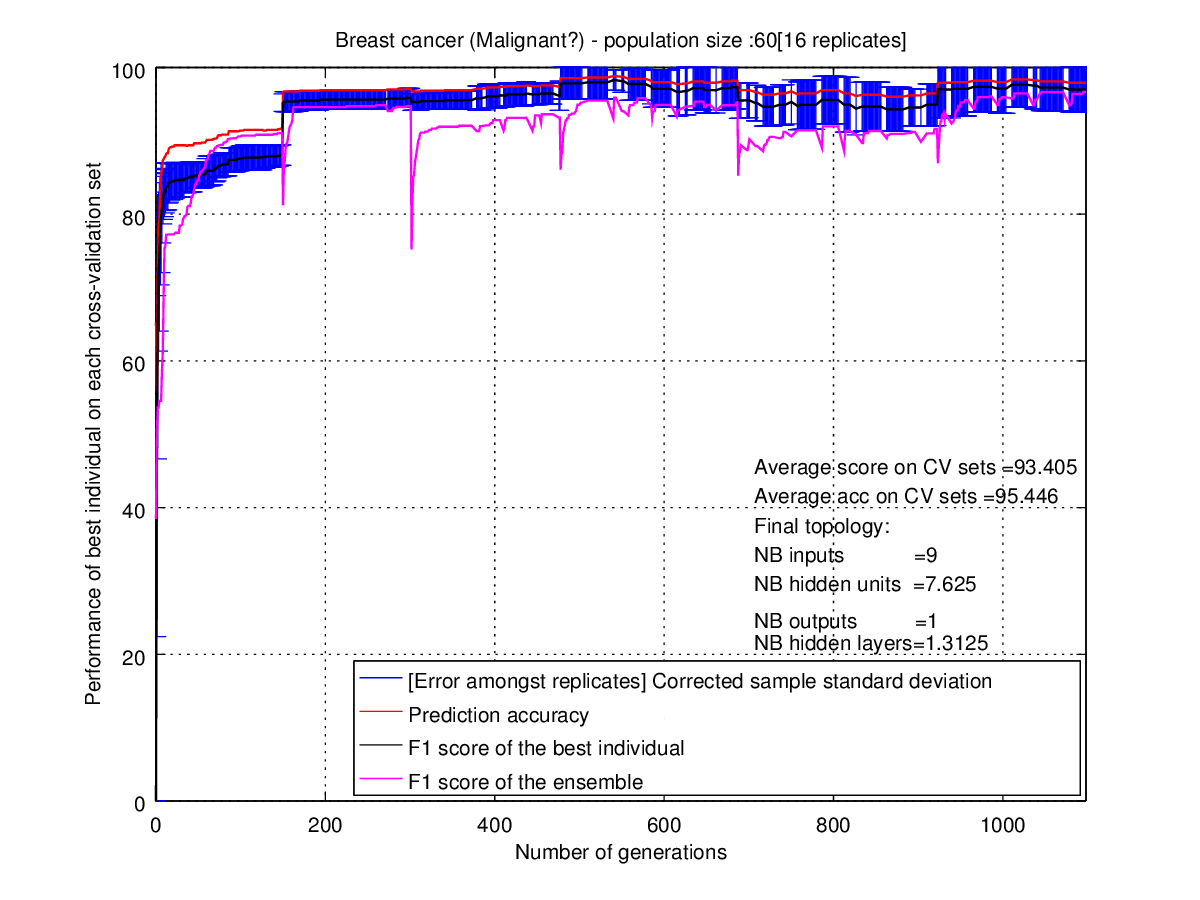
\includegraphics[scale=0.7]{malignant-performancesVSepochs-DE-derived-rand}
  \vspace{-12pt}
  \caption{Convergence towards optimal solution (DE derived termination criteria)}
  \label{malignant-perfs-DE-derived-rand}
\end{figure}

\begin{figure}[h]
  \centering
  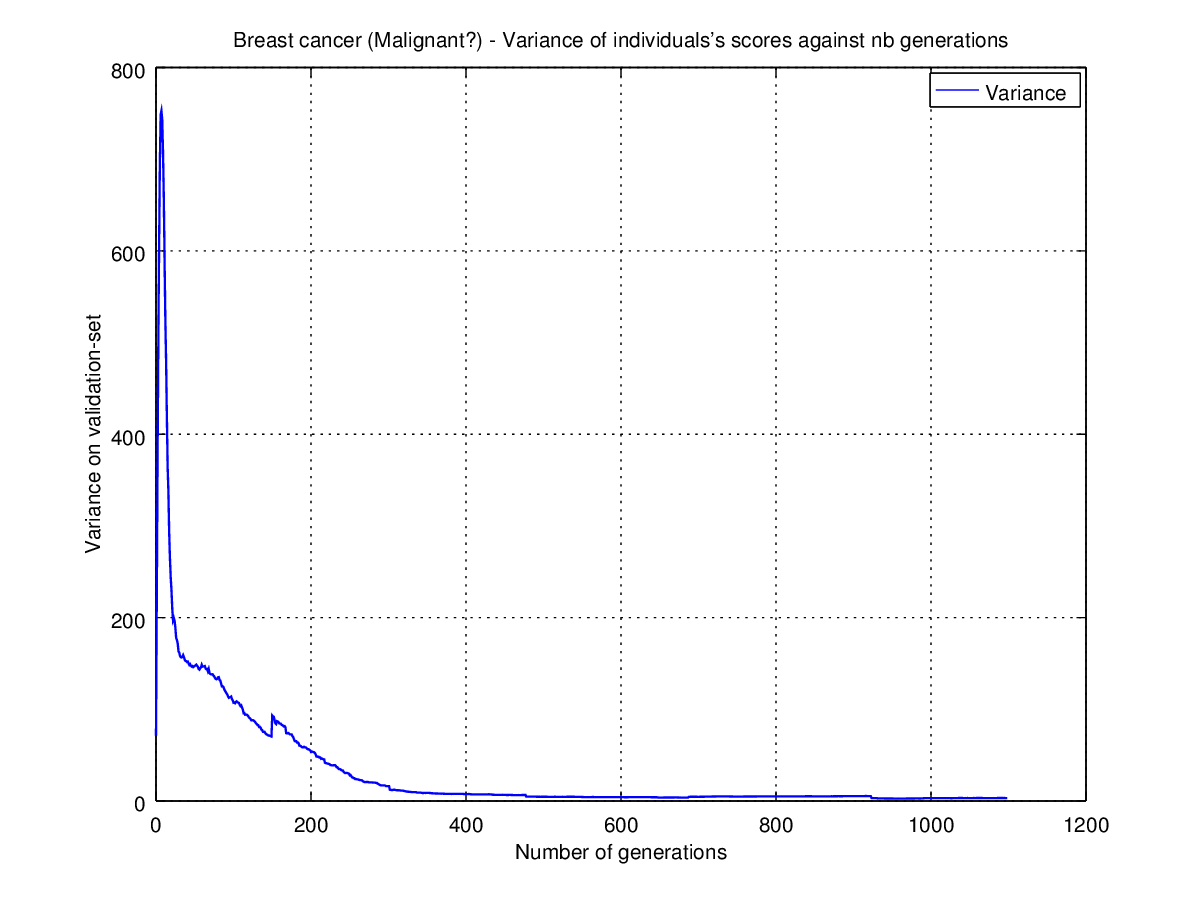
\includegraphics[scale=0.7]{malignant-varianceVSepochs-DE-derived-rand}
  \vspace{-12pt}
  \caption{Convergence towards optimal solution (DE derived termination criteria)}
  \label{malignant-variance-DE-derived-rand}
\end{figure}

\begin{figure}[h]
  \centering
  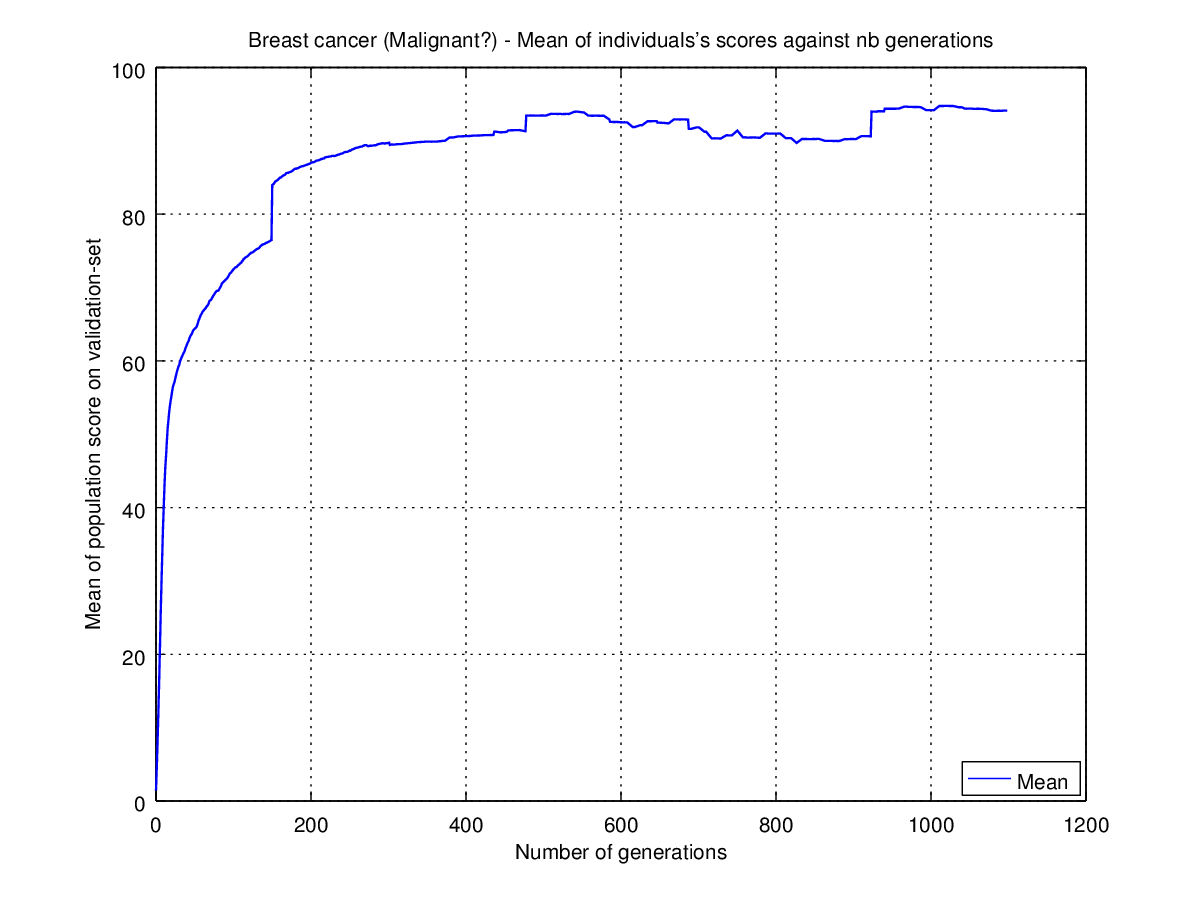
\includegraphics[scale=0.7]{malignant-meanVSepochs-DE-derived-rand}
  \vspace{-12pt}
  \caption{Overall population gets fitter (Mean, DE derived termination criteria)}
  \label{malignant-mean-DE-derived-rand}
\end{figure}

\clearpage

\section{Measurement Methodology}

Because of the inherent randomness of Genetic Algorithms a plot of a single run is not enough to make any conclusion. In order to capture the performance of the algorithm, each result is averaged over a number of replicates (10 to 16 replicates depending on the experiment). 
\\ \\
To address the problem of measuring random-based and stochastic algorithms, the following logic is followed. For each generation, the \textit{Corrected Sample Standard Deviation} of the best score amongst all replicates is calculated and plotted using error bars. Since each run is executed with a different random seed, this give an indication of the range of values in which the algorithm is likely to perform no matter what the initial weights of the individuals. 
\\ \\
Regarding the metrics displayed in the annotations of the performance plots, the accuracy and score values are calculated using the the cross-validation (to stay consistent with the initial effort of evaluating a model by its ability to generalize to new data). After selecting the trained model, these two values are calculated by averaging the performances of the trained model on each validation fold.


\section{Experiment Replicability}

Training a neural network initially involves setting the weights to random values. Moreover, the algorithms used in this research project are stochastic and also involeusing random values. In order for this experiment to be replicated, the logic of Algorithm \ref{pseudocode-seed-settings} must be followed to set the seeds of the random number generator.

\begin{algorithm}[H]\small
  \caption{Seed settings}\label{pseudocode-seed-settings}
  \begin{algorithmic}[1]
    \State $\dots$
    \For{$i = 0 \to nb replicates$} 
      \State $set seed(i \times 10$)
      \State $results(i) \gets optimize(\dots)$
    \EndFor
    \State $average\_results(results)$
    \State $\dots$
  \end{algorithmic}
\end{algorithm}

\newpage

\section{Comparison with previous work}

\begin{table}[h]
  \begin{center}
    \begin{tabular}{ | p{15cm} | l |}
    \hline
    Technique & Accuracy (\%) \\ \hline
    Four Layer Perceptron                 &   81.39  \\ \hline
    Radial Basis Function                 &   87.42  \\ \hline
    Probabilistic Neural Network          &   71.08  \\ \hline
    Self Organising Map                   &   80.69  \\ \hline
    Support Vector Machines               &   95.58  \\ \hline
    k Nearest Neightbors                  &   94.28  \\ \hline
    Naïve Bayes                           &   91.87  \\ \hline
    Hybrid ANN/GA (Fixed topology)        &   93.58  \\ \hline
    Partially Connected Neural Network    &   81.08  \\ \hline 
    \hline
    \hline
    Cooperative co-evolution              &   95.63  \\ \hline
    Multisurface Method Tree              &   97.00  \\ \hline
    \hline
    \hline
    Hybrid ANN/Particle Swarm Optimization  (max topology: 18 units per hidden layer, 2 hidden layers)               &   93.08  \\ \hline
    Hybrid ANN/Differential Evolution       (max topology: 18 units per hidden layer, 2 hidden layers)               &   95.45  \\
    \hline
    \end{tabular}
  \end{center}
  \vspace{-10pt}
  \caption{Results against state-of-the-art methods on Breast Cancer Wisconsin (Diagnostic). Source: \cite{Gorunescu-2014}}
  \label{table:state-of-the-art-comparison}
\end{table}

No result within table \ref{table:state-of-the-art-comparison} can be directly compared with Hybrid ANN/PSO and Hybrid ANN/DE since in the case of the coevolution of weights \textit{and} topology the search space is substantially larger. Nevertheless, it can be appreciated that both PSO and DE offer results comparable to these well established methods. The results obtained by the hybrid ANN/DE show that for the Breast Cancer Wisconsin (Diagnostic) data set, state-of-the-art ANNs can be approached. These results should be appreciated knowing that the Hybrid ANN/PSO and Hybrid ANN/DE have been trained on \textit{cleaned} data where samples with missing data have been removed whereas the cooperative co-evolution and multisurface method three used a complete data-set.

\clearpage

\chapter{Evaluation}

Even Though the initial goal of using a canonical genetic algorithm appeared not to work for training ANNs, all the objectives of section \ref{section:aims-and-objectives} were met. This project involved a significant amount of personal research and self learning.\\

Multiple interesting data-sets were found thanks to the UCI Machine Learning repository \cite{uci-machine-learning-repo-2013}. \textit{Data analytics} and \textit{Computational Intelligence} university courses were undertook as well as a \textit{Machine Learning} online course. A neural network implementation that can adopt any given topology was written in C++ based on simple linear algebra. DE and PSO have been implemented in order to evolve a population of neural networks with diverse topologies. An elective scheme was implemented for the population of neural networks to observe whether the population as an ensemble made better prediction than the single best model alone. Finally a simple statistical analysis using multiple replicates, error bars as well as mean and variance of the fitness of the individuals was added to the implementation. The statistics show that DE produces excellent performances in training neural networks.
\\ \\
In terms of planning, most of the background in biology-inspired computing and justification of chosen techniques was accomplished in the first 4 months. I used the temporary absence of supervision in November and December to choose an adequate programming language, deciding on the best approach to implementating the ANN and reading publications. the period from early January until April was an implementation and dissertation writing phase where I initially struggled working with a real number encoding GA to train ANNs and questionned whether the combination of Gradient Descent/Backpropation would be interesting to implement. I then implemented DE which led me to implementing the benchmark and calculating all the appropriate statistics in order to assert that the algorithm is functional along with the plotting script. Finally I implemented PSO and the elective scheme for ANN ensembles. Overall I judge this project as well managed, even though the initial goals were ambitious and all estimated deadlines were not met, I used these deadlines as guidance more than anything. Above all, I think that the consistency of my work ethic counterbalanced this problem.
\\ \\
I am pleased with the fact that my work approaches the performances of the leading edge machine learning techniques even though my program evolves the topology autonomously. Above the fact that all the initial goals were met, this is also why I evaluate this project as a success. Driven by the enthusiasm to build a useful and interesting piece of work, I set myself beginning of the year a personal goal of making a relevant contribution to the scientific community over the next 12 months. I am grateful that one of the main outcomes of this project is its continuity towards a research internship, which should lead to seeing this work published.

\chapter{Conclusions}

It was remarked that using neural networks as predictive model requires some additional set-up such as \textit{feature-scaling}. It was experienced that using more intelligent fitness functions and maintaining the imbalance-ratio in each cross-validation fold helped dealing with problems such as imbalanced data-sets.
\\ \\
The experiment shows that using EAs to evolve neural networks is a feasible method to obtain ANNs approaching state-of-the-art performances ont the \textit{Breast Cancer Wisconsin for Diagnosis} with about 97\% accuracy \cite{Gorunescu-2014}. This is provided that the crossover operation is not to brutal. The use of a canonical GA with a one point crossover is destructive in most cases therefore an optimization method such as Differential Evolution or Particle Swarm Optimization is more suitable. The experiment also shows that EAs allow simultaneous search of topology and weights easily. Something that isn't achievable using the Back Propagation algorithm with a Gradient based optimization algorithm.
\\ \\
Multiple limitations were noticed. Because of the inherent randomness of EAs, they do not guarantee any improvement from a generation to the next. It is also well known that an EA based optimization algorithm will be slower than a gradient-based approach. Another constraint present in the current implementation of both DE and PSO is that a maximum topology must be chosen to limit the length of the genome. Another limitation for DE is the arbitrary choice of parameters (the convergence rule is applied for PSO). What is assumed is that the parameters of DE values might not be suitable for all problem. 
\\ \\
Potential solutions to reach full automation include meta-heuristic and hyper-heuristic algorithms in order to pre-tune the optimization algorithm. This means that the learning process is not fully automated. It was noticed that DE tends to be a generally efficient global search algorithm without any premature optimisation problem. In every single problem (Breast Cancer Wisconsin Diagnostic, Breast Cancer Recurrence and Haberman's survival) DE shows signs of continuous learning throughout the different validation sets, which isn't as true for PSO. PSO tends to have a very quick learning rate and see the population converge quickly towards a solution. In essence, this phenomenon demonstrates good local search abilities. However, in the context of a cross-validated training, this often leads to PSO being stuck in a local optima due to the whole population converging quickly towards the global optima of the current validation fold.
\\ \\
Finally, the predictive ability of the ANN ensemble was observed. It was noticed that the ensemble tends to show signs of overfitting as the performances obtained from a validation fold to the next are often poorer than the ones on the current validation fold.

\newpage

\section{Further Study}

\subsection{Speciation}

A method called \textit{speciation} speciation consist of simultaneously evolving subpopulations (species) of individuals that are close in nature. In the context of ANNs, this means simultneously evolving subpopulations of ANNs which have similar topologies. Since each speciated subpopulation are all \textit{neighbors} it is a way to introduce one or more local searches in order to speed-up the learning process. Speciation techniques have been previously used \cite{stanley-2002}.

\subsection{Hybrid optimization algorithms}

Optimization algorithms have advantages and disadvantages, for example the Back-Propagation algorithm converges fast but requires a provided topology and can fall in a local minima. Evolutionary algorithms can evolve both the topology and the weights of Neural nets but because of their inherent randomness, they tend to be slower. A combination of the backpropagation algorithm with an Evolutionnary approach would be interesting to investigate in order to obtain an hybrid optimization algorithm that evolves both the topology and the weights faster. Such hybrid algorithms have been researched however it is still hard to know whether it is worth implementing such algorithm for a given therefore a research involving a wide range of problem of different complexity would be interesting to explore. Hybrid optimization algorithms have been previously researched \cite{yao-1999}.
\\ \\
It was observed that PSO was a very efficient local search algorithm, Whereas DE was a naturally good global search algorithm. Since both of these are EAs, population based and therefore close in nature, it would be interesting to build a hybrid of these two with the advantages of both. Also a differential evolution with global and local neighborhoods search could be explored.

\subsection{Fitness penalties to guide Differential Evolution}

The use of different fitness penalties to help DE find a more suitable solution would be worth exploring. For example, one could implement a penalty equal to the total number of neuron in the network (normalized) in order to guide DE towards the smallest possible topology.

\subsection{Neural Network Ensembles}

Differential evolution has the benefit of creating a highly diverse population. In this project the goal given to the algorithm was to find a best neural network. Essentially, this means training the ensemble as a whole by replacing the fitness function to the one used to compute the score of the ensemble. It would be interesting the obtained result was an algorithm that requires a lesser amount of generations. As confirmed by Yao \cite{yao-1999} Neural Network Ensembles have been previously researched.

\subsection{Comparing Genetic Algorithm and Artificial Immune Systems as optimization algorithms}

Artificial Immune Systems (AIS) as optimization algorithm or classifiers have been researched for less time than EAs, since AIS as opposed to GAs have a multi-modal behaviour, it would be interesting to compare the performances of the two on a range of problems.

\subsection{Comparison with the NEAT method}

The Neat method \cite{stanley-2002} is a close candidate for comparing this method. The NEAT method uses two genomes representing a not-fully-connected neural network and a genetic algorithm to evolve the topology and weight values of an ANN. Observing the different behaviour of the NEAT method to my work would inform us about how good my method is. 

\subsection{Coevolution of topology and weight of Multitask neural networks}

Training neural networks on multiple \textit{related} data sets (also known as Multitask Learning: MTL) has been explored using the backpropagation algorithm. It would be very interesting to explore the use of a technique like Differential Evolution to evolve the topology and weights of the MTL network. The expected result would be a much more \textit{adaptive} optimization algorithm.


\subsection{Investigation on a wider range of problems}

In this research project, all the problems tackled were diseases. Since the current implementation of an EA-based optimizer and a neural network can be applied to any bi-classification problem, it would be interesting to extend this investigation to problems of different nature. Solving multi-classification problem such as the digit recognition problem would also be interesting since it would allow me to more easily compare my results with an existing publication.

%
% appendices
%
 
\newpage

\appendix
\chapter{Data Set resources} \label{App:AppendixA-data set-resources}

One of the goals of this project is to build a system that will autonomously generate an ANN with the appropriate topology. Therefore, it is important to use multiple data sets in order to observe whether or not the topology of the obtained ANN is different for each problem. In order to make sure that the results can be easily replicated and compared, all used data sets come from an open source repository.

\subsection{Data quality}

The class attribute is always set as the last column in all data sets used in this project without exception. Attributes with no correlations have been removed and fields containing missing attributes have been removed or replaced by \textit{most-frequent} when judged adequate. However fields with multiple missing attributes values have been removed by default. The data cleaning was done using OpenRefine and Tableau was used to produce the visualisation.


\begin{figure}[h]
  \centering
  \begin{minipage}[h]{0.4\textwidth}
    \subsubsection{Breast Cancer Wisconsin (Diagnostic)}
    \textbf{Attributes:}
      \begin{enumerate}
        \setlength\itemsep{0.001em}
        \item Sample code number (id number)
        \item Clump Thickness (1 - 10)
        \item Uniformity of Cell Size (1 - 10) 
        \item Uniformity of Cell Shape (1 - 10) 
        \item Marginal Adhesion (1 - 10) 
        \item Single Epithelial Cell Size (1 - 10) 
        \item Bare Nuclei  (1 - 10) 
        \item Bland Chromatin (1 - 10) 
        \item Normal Nucleoli (1 - 10) 
        \item Mitoses (1 - 10)
        \item Severity
          \begin{enumerate}
            \item 2 = Benign
            \item 4 = Malignant
          \end{enumerate}
      \end{enumerate}

      Corresponding University of California Irvine description \href{https://archive.ics.uci.edu/ml/datasets/Breast+Cancer+Wisconsin+\%28Diagnostic\%29}{here}. \cite{uci-machine-learning-repo-2013}
  \end{minipage}
  \hfill
  \begin{minipage}[h]{0.5\textwidth}
    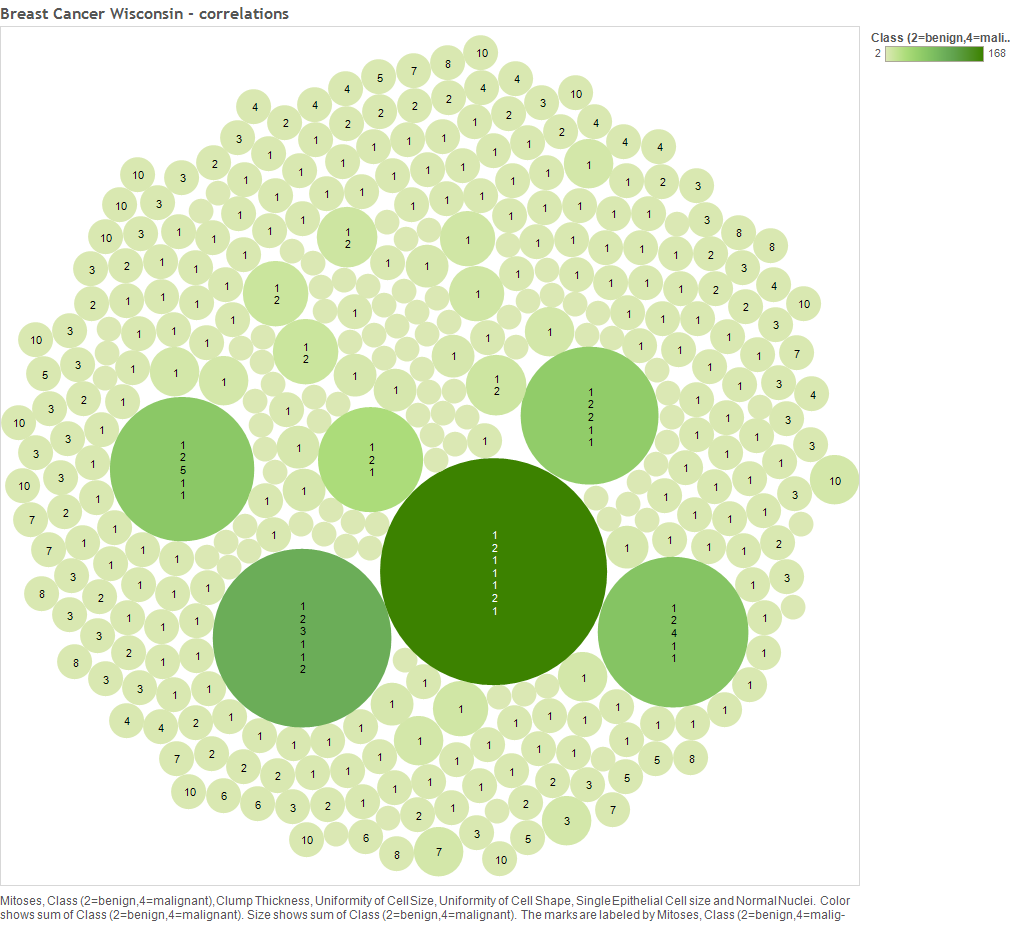
\includegraphics[scale=0.3] {Breast_cancer_Wisconsin_Visualisation}
    \caption {Instances of the breast cancer data set. Visualisation of common-features with identical severity}
    \label{breast-cancer-visualization}
  \end{minipage}
  \caption{Breast cancer diagnosis data set description}
  \label{breast-cancer-diagnosis-data set-description}
\end{figure}

\begin{figure}[h]
  \centering
  \begin{minipage}[h]{1.0\textwidth}
    \subsubsection{Haberman's survival}
    \textbf{Attributes:}
    \begin{enumerate}
      \setlength\itemsep{0.001em}
      \item Age of patient at time of operation (numerical)
      \item Patient's year of operation (year - 1900, numerical) 
      \item Number of positive axillary nodes detected (numerical) 
      \item Survival status (class attribute) 
        \begin{enumerate}
          \item 1 = the patient survived 5 years or longer
          \item 2 = the patient died within 5 year
        \end{enumerate}
    \end{enumerate}

    Corresponding University of California Irvine description \href{https://archive.ics.uci.edu/ml/datasets/Haberman\%27s+Survival}{here}. \cite{uci-machine-learning-repo-2013}    
  \end{minipage}
  \hfill
  \begin{minipage}[h]{0.0\textwidth}
    % no visualisation yet ?
  \end{minipage}
  \caption{ Haberman's survival data set description}
  \label{ haberman-data set-description}
\end{figure}

\begin{figure}[h]
  \centering
  \begin{minipage}[h]{1.0\textwidth}
    \subsubsection{Breast Cancer: Recurrence or Not}
    \textbf{Attributes:}
      \begin{enumerate}
        \setlength\itemsep{0.001em}
        \item age: 0 for 10-19, 1 for 20-29 ... 8 for 90-99
        \item menopause: 0 for lt40, 1 for ge40, 2 for premeno
        \item tumor-size: 0 for 0-4, 1 for 5-9 ... 11 for 55-59
        \item inv-nodes: 0 for 0-2, 1 for 3-5 ... 12 for 36-39
        \item node-caps: 0 for no, 1 for yes
        \item deg-malig: 0 for 1, 1 for 2, 2 for 3
        \item breast: 0 for left, 1 for right
        \item breast-quad: 0 for left-up, 1 for left-low ... 4 for central
        \item irradiat: 0 for no, 1 for yes
          \begin{enumerate}
            \item 0 = No reccurence event
            \item 1 = Recurrence events
          \end{enumerate}
      \end{enumerate}

      Related University of California Irvine description \href{https://archive.ics.uci.edu/ml/datasets/Breast+Cancer}{here}. From the Institute of technology, Ljubljana Yugoslavia \cite{uci-machine-learning-repo-2013}.
  \end{minipage}
  \hfill
  \begin{minipage}[h]{0.0\textwidth}
    % no visualisation yet ?
  \end{minipage}
  \caption{Data set description: Breast Cancer: Malignant or Benign}
  \label{mammographic-mass-screaning-data set-description}
\end{figure}

\begin{figure}[!th]
  \centering
  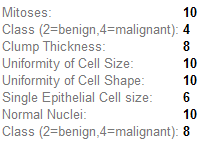
\includegraphics[scale=1] {Breast_cancer_Wisconsin_Visualisation_legend}
  \caption {Legend of Figure \ref{breast-cancer-visualization}}
  \label {breast-cancer-visualization-legend}
\end{figure}


\chapter{Results - Breast Cancer: Recurrence or Not ?} \label{complementary-results-recurrence}


\subsection{Differential Evolution (mutation scheme: DE/RAND)}

\begin{figure}[h]
\centering
  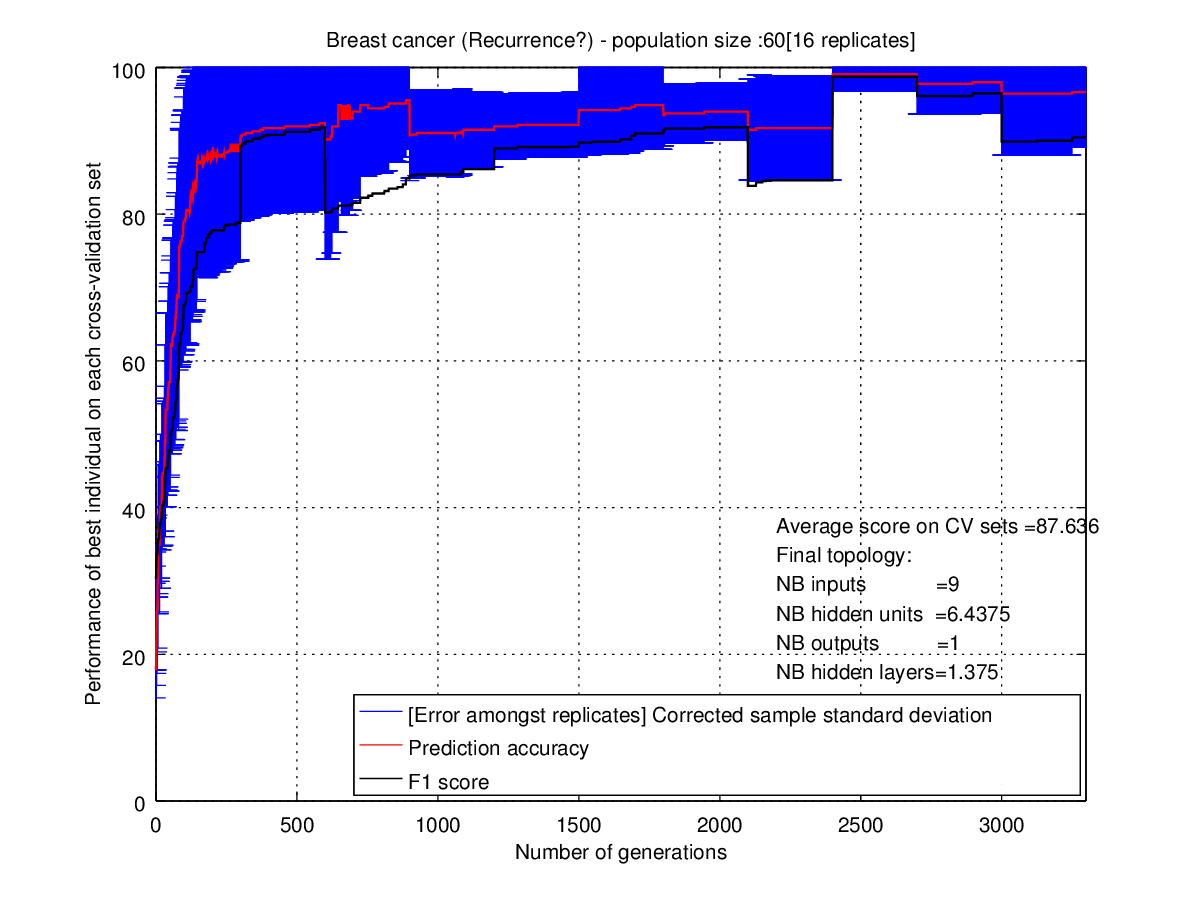
\includegraphics[scale=0.65]{recurrence-performancesVSepochs-DE}
  \vspace{-12pt}
  \caption{Optimization of the neural network population (DE/rand)}
  \label{recurrence-perfs}
\end{figure}
\vspace{-10pt}

\begin{figure}[h]
\centering
  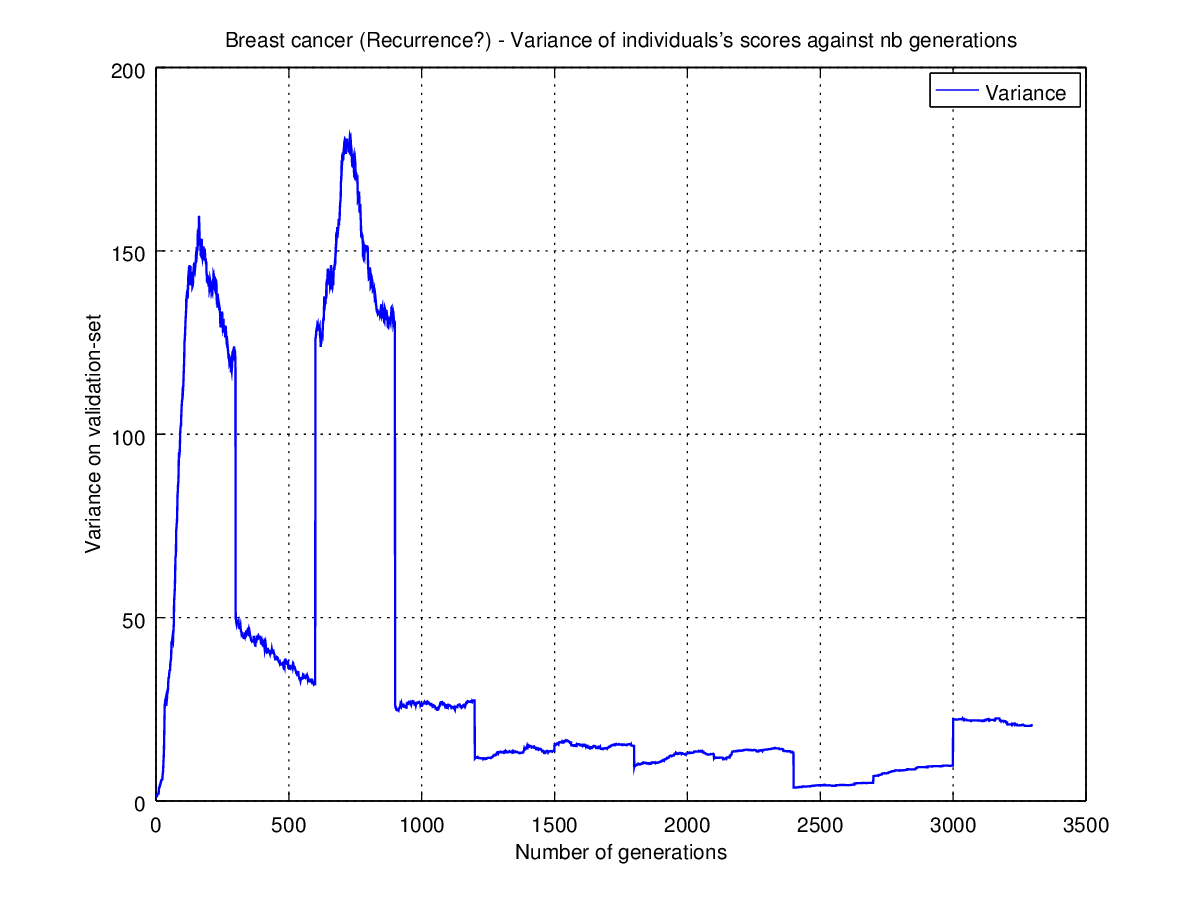
\includegraphics[scale=0.65]{recurrence-varianceVSepochs-DE}
  \vspace{-12pt}
  \caption{Convergence towards optimal solution}
  \label{recurrence-variance}
\end{figure}
\vspace{-10pt}

\clearpage

\subsection{Differential Evolution (mutation scheme: DE/BEST)}

\begin{figure}[h]
  \centering
  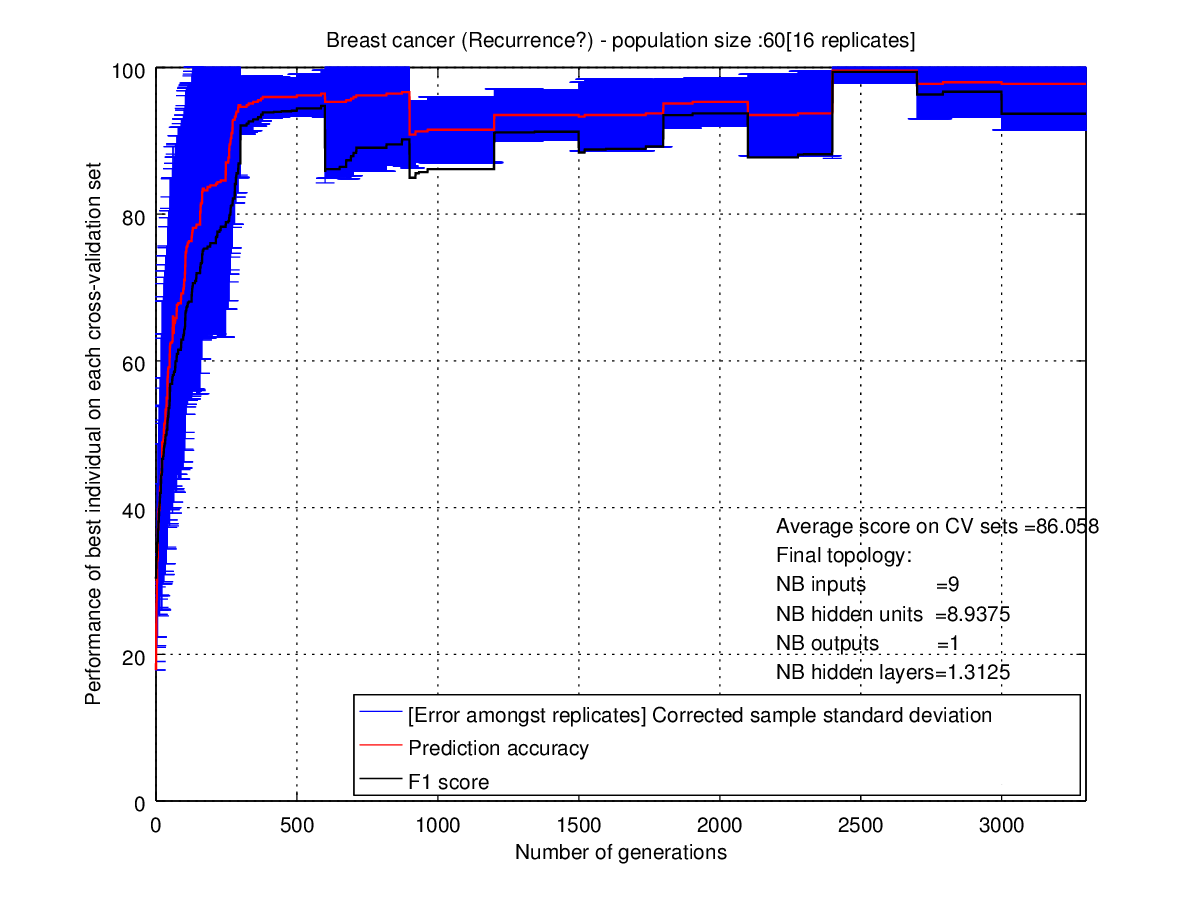
\includegraphics[scale=0.7]{recurrence-performancesVSepochs-DE-BEST}
  \vspace{-12pt}
  \caption{Learning pace}
  \label{recurrence-perfs}
\end{figure}

\begin{figure}[h]
  \centering
  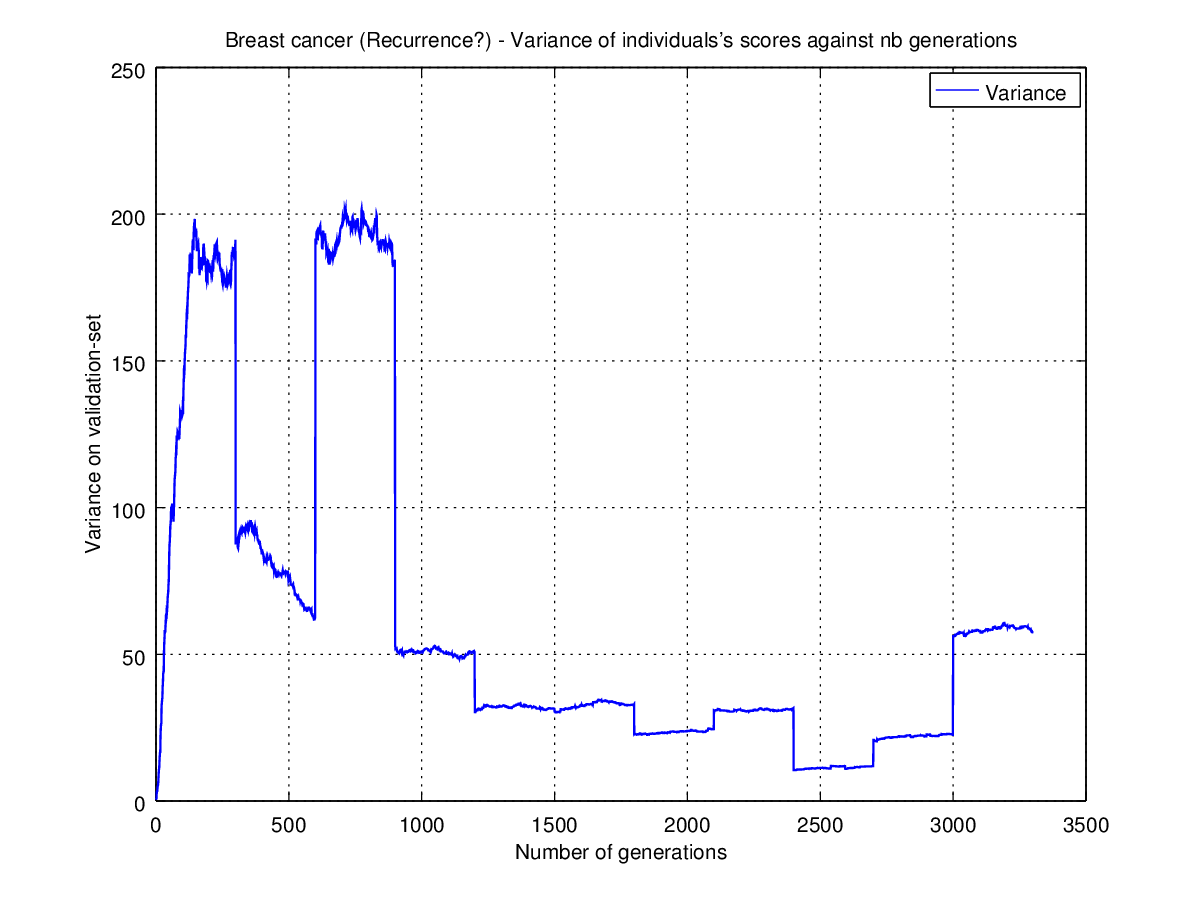
\includegraphics[scale=0.7]{recurrence-varianceVSepochs-DE-BEST}
  \vspace{-12pt}
  \caption{Convergence towards optimal solution}
  \label{recurrence-variance}
\end{figure}

\clearpage

\begin{figure}[h]
  \centering
  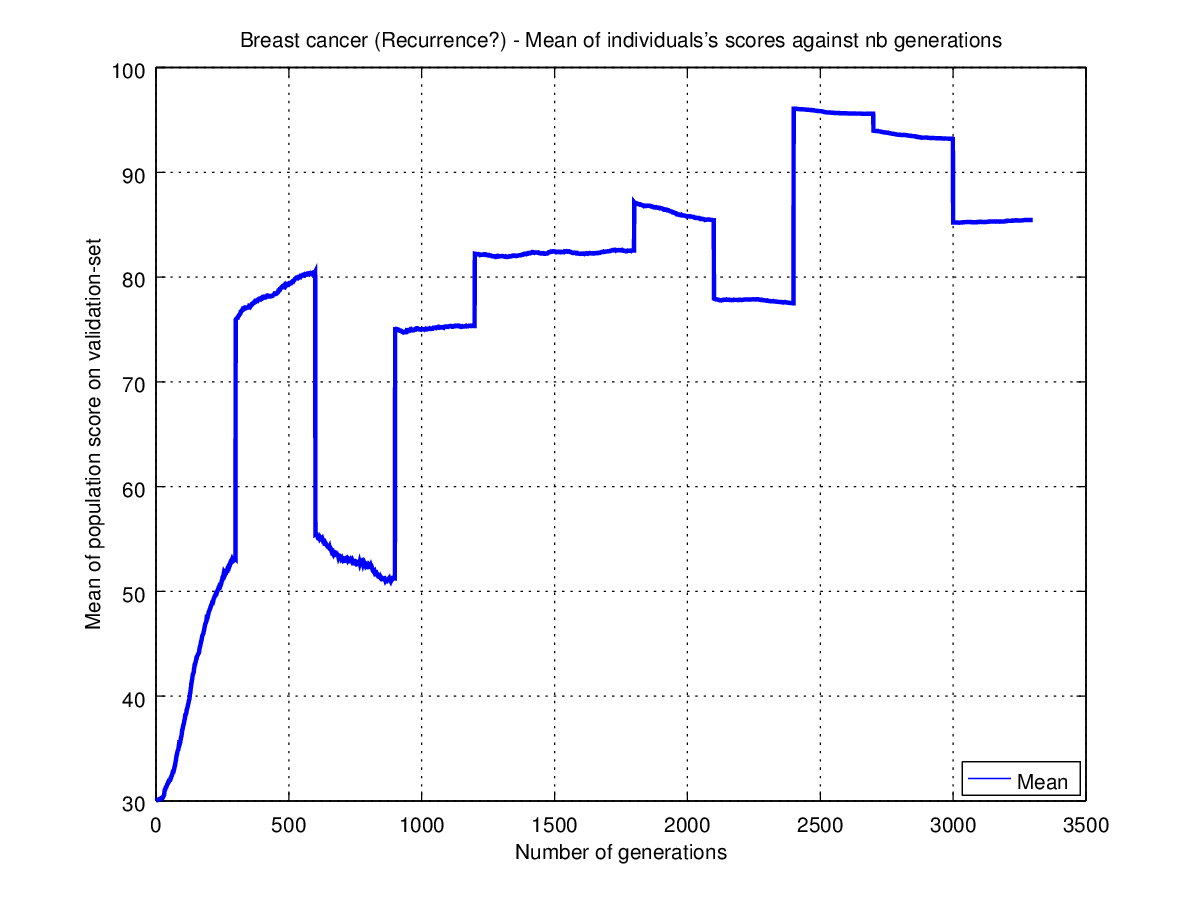
\includegraphics[scale=0.7]{recurrence-meanVSepochs-DE}
  \vspace{-12pt}
  \caption{Mean of the scores of the individuals}
  \label{recurrence-mean-DE}
\end{figure}

\clearpage

\subsection{Particle Swarm Optimization}

\begin{figure}[h]
  \centering
  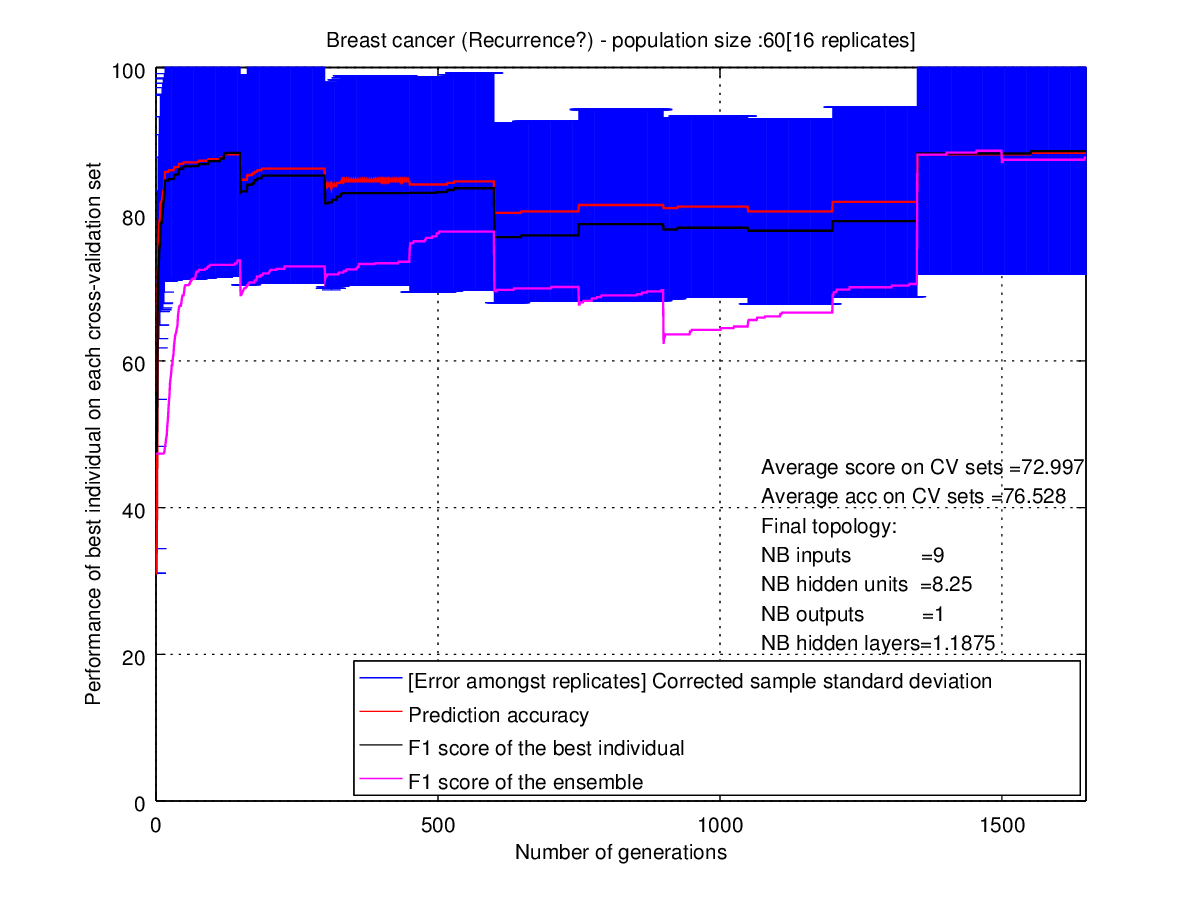
\includegraphics[scale=0.7]{recurrence-performancesVSepochs-PSO}
  \vspace{-12pt}
  \caption{Optimization of the neural network population (PSO)}
  \label{recurrence-perfs-PSO}
\end{figure}

\begin{figure}[h]
  \centering
  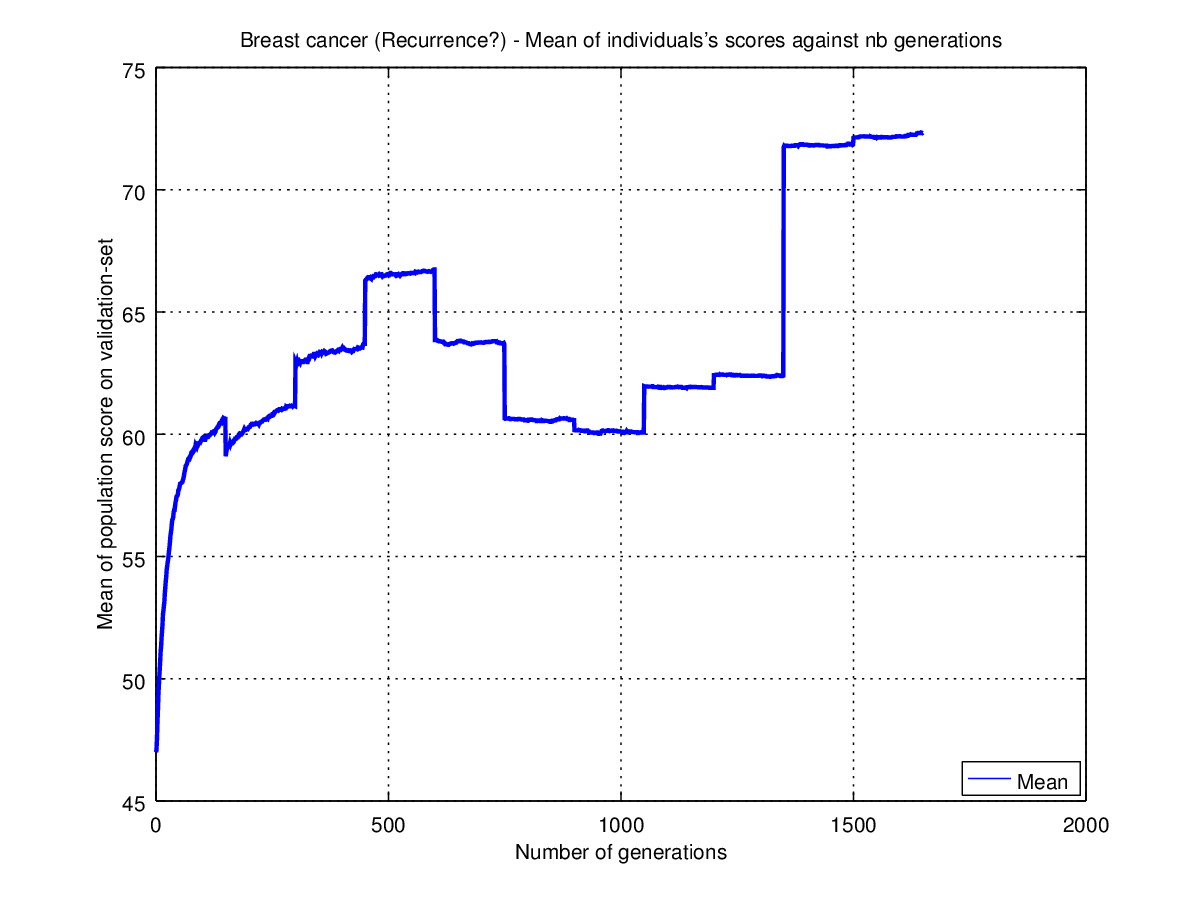
\includegraphics[scale=0.7]{recurrence-meanVSepochs-PSO}
  \vspace{-12pt}
  \caption{Mean of the scores of the individuals (PSO)}
  \label{recurrence-mean-PSO}
\end{figure}

\clearpage

\begin{figure}[h]
  \centering
  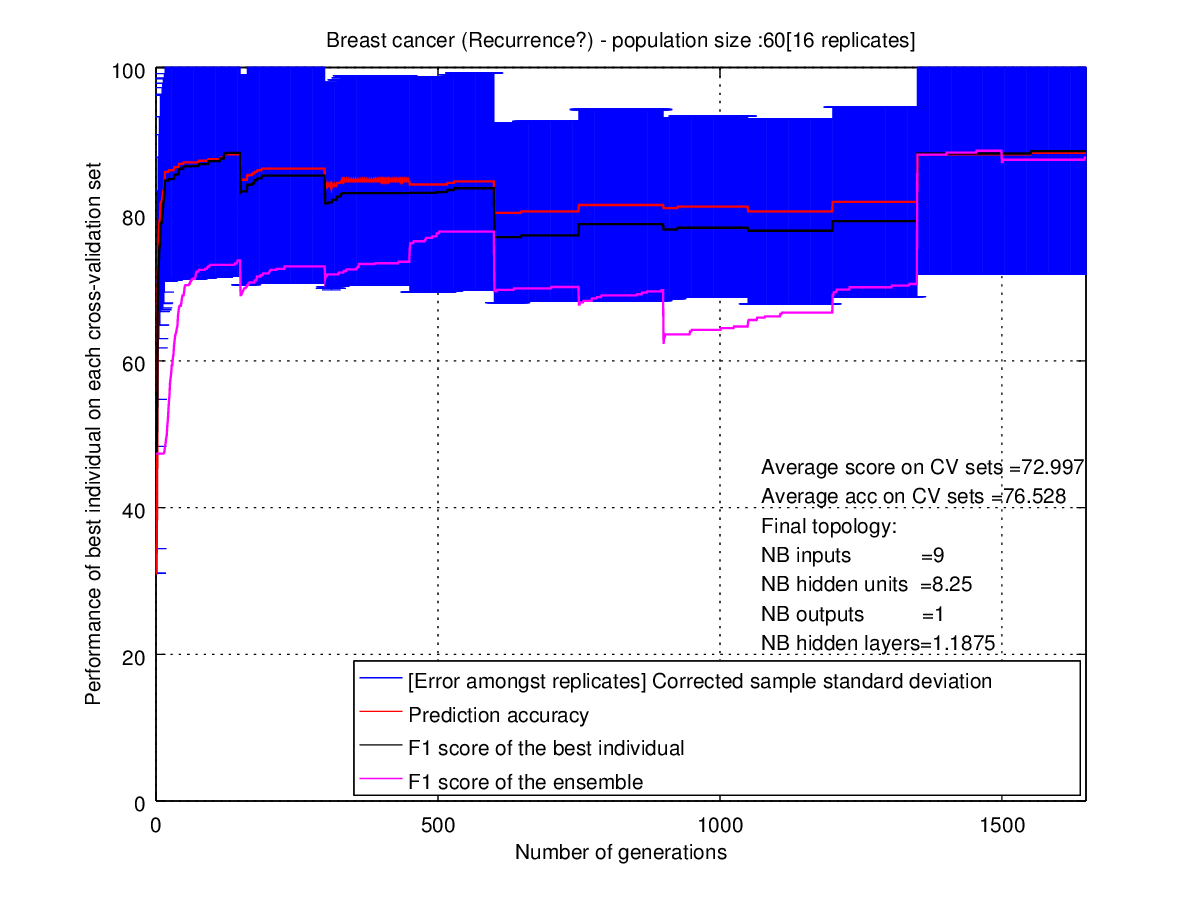
\includegraphics[scale=0.7]{recurrence-performancesVSepochs-PSO}
  \vspace{-12pt}
  \caption{Optimization of the neural network population (PSO)}
  \label{recurrence-perfs-PSO}
\end{figure}

\clearpage

\chapter{Haberman's survival test} \label{complementary-results-haberman}

\subsection{Differential Evolution (mutation scheme: DE/RAND/1)}

\begin{figure}[h]
  \centering
  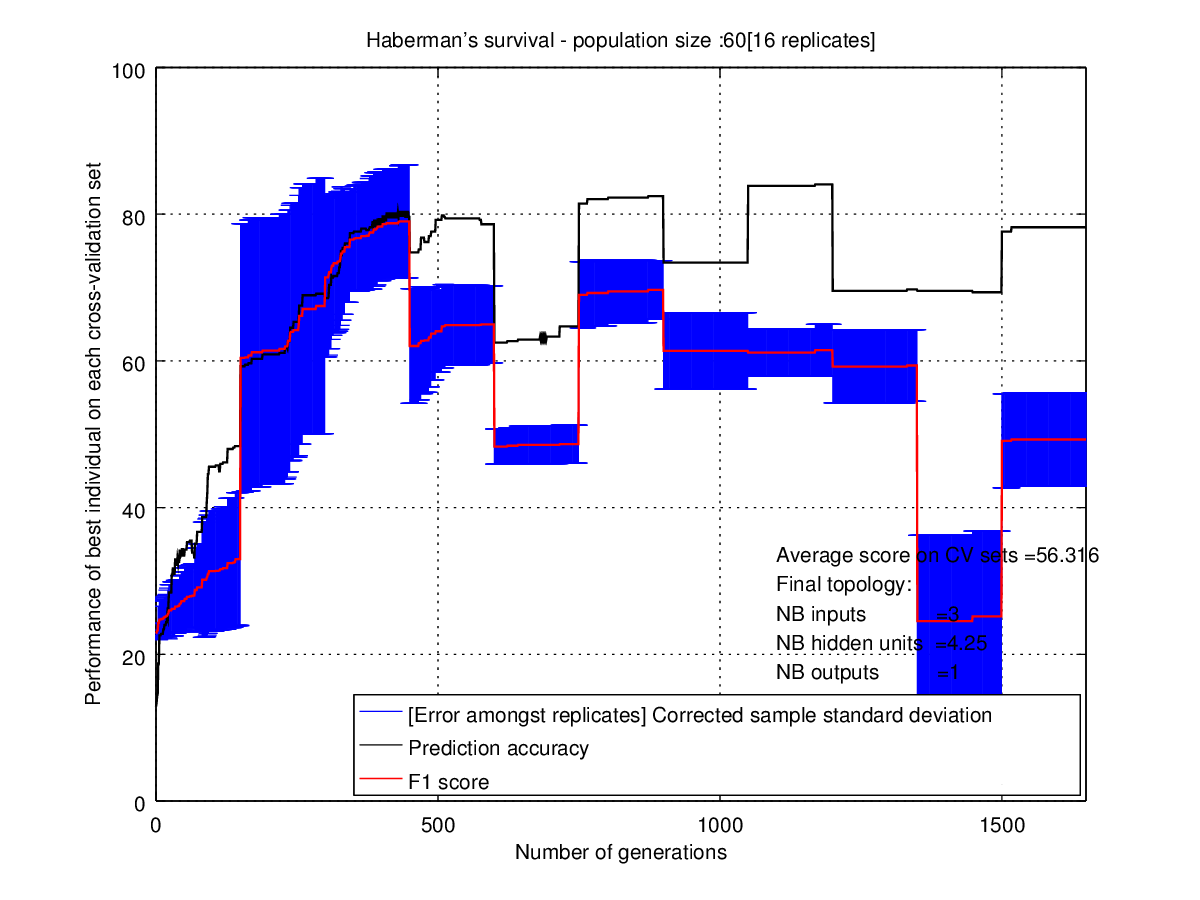
\includegraphics[scale=0.65]{haberman-performancesVSepochs-DE}
  \vspace{-12pt}
  \caption{Optimization of the neural network population (DE/rand)}
  \label{haberman-perfs-DE-rand}
\end{figure}
\vspace{-10pt}

\begin{figure}[h]
  \centering
  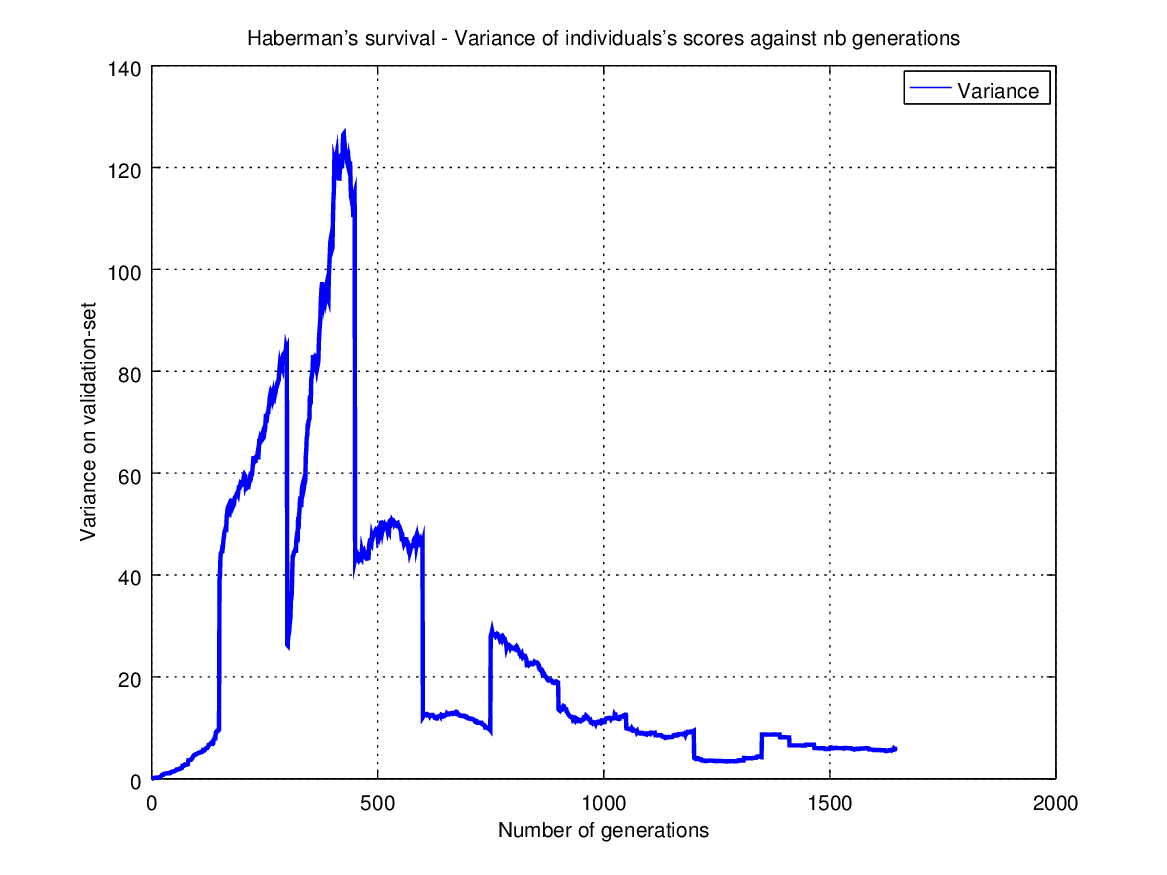
\includegraphics[scale=0.65]{haberman-varianceVSepochs-DE}
  \vspace{-12pt}
  \caption{Convergence towards optimal solution}
  \label{haberman-variance-DE-rand}
\end{figure}
\vspace{-10pt}

\clearpage

\subsection{Differential Evolution (mutation scheme: DE/BEST/1)}

\begin{figure}[h]
  \centering
  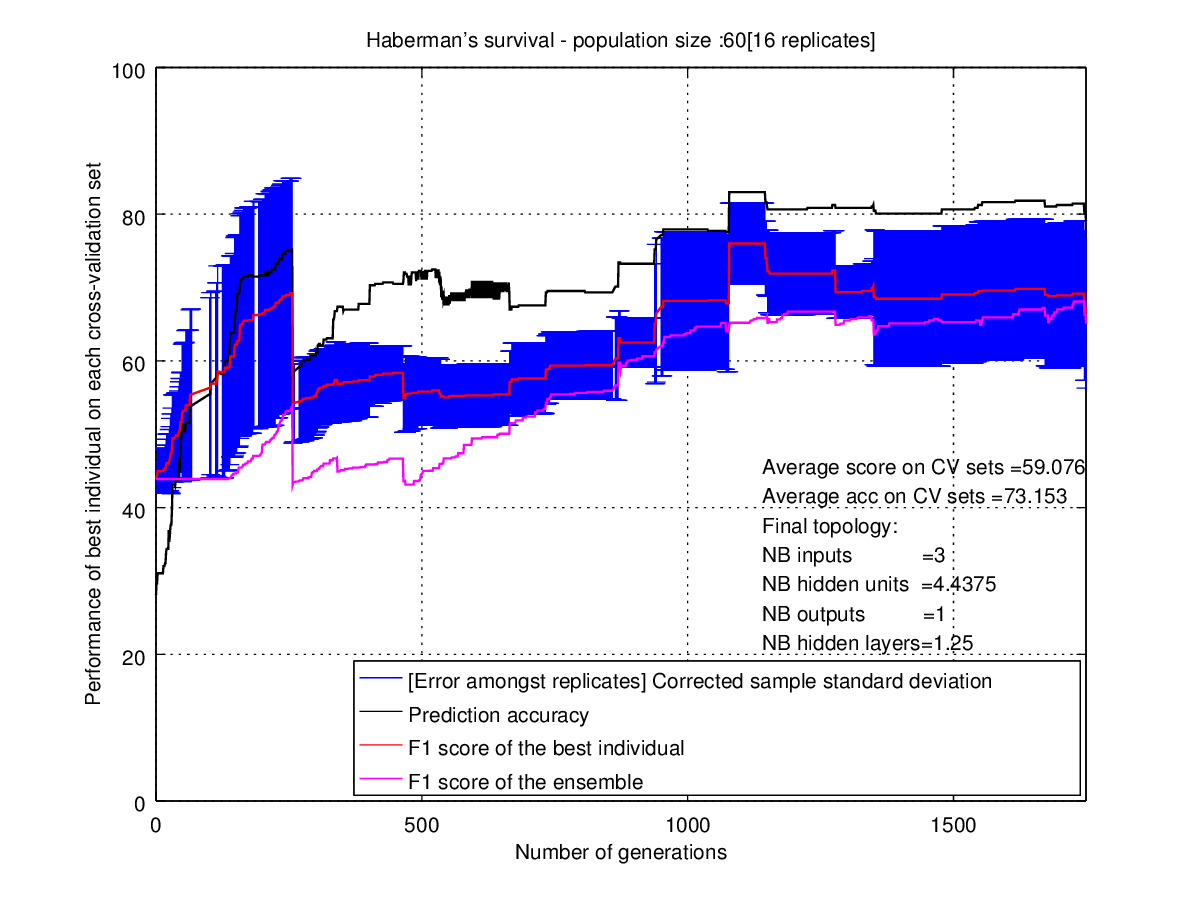
\includegraphics[scale=0.7]{haberman-performancesVSepochs-DE-BEST}
  \vspace{-12pt}
  \caption{Optimization of the neural network population (DE/best)}
  \label{haberman-perfs-de-rand}
\end{figure}

\begin{figure}[h]
  \centering
  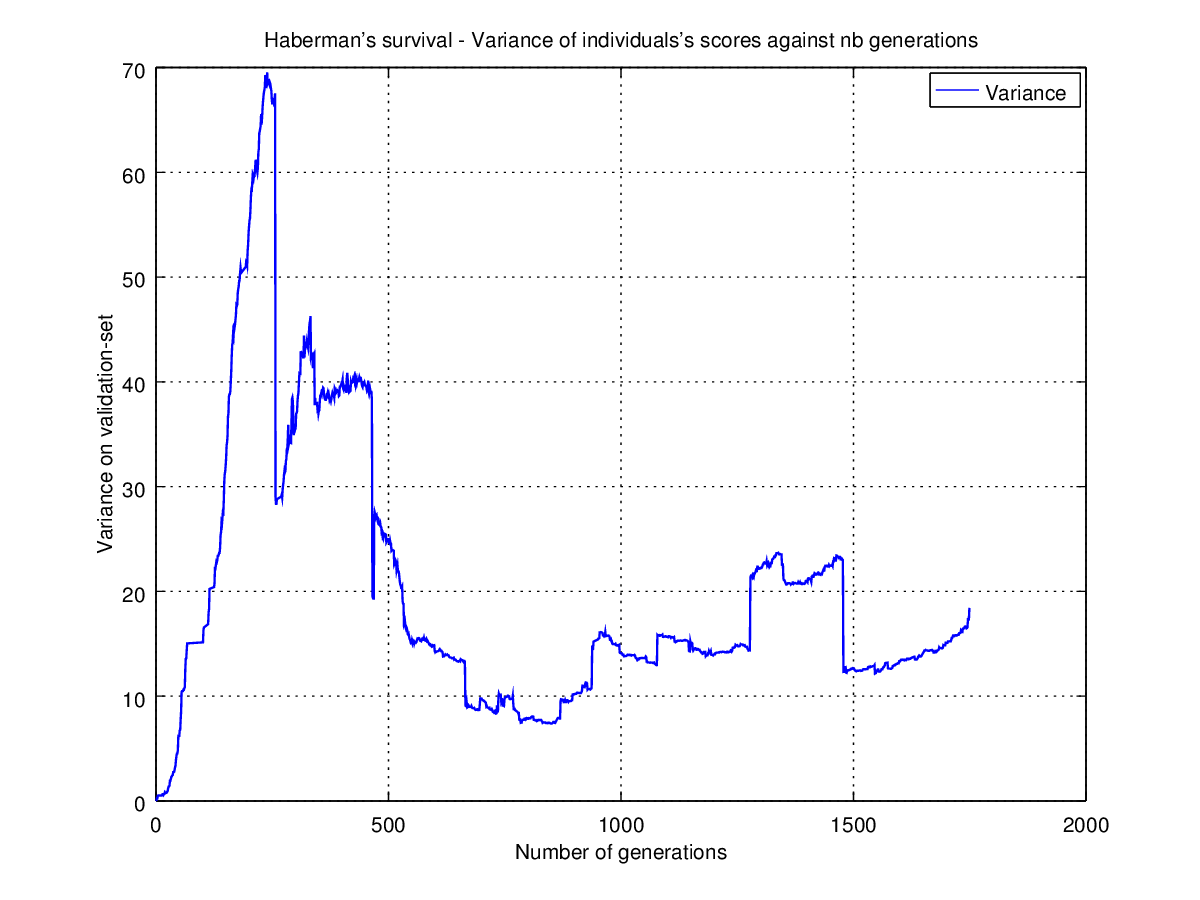
\includegraphics[scale=0.7]{haberman-varianceVSepochs-DE-BEST}
  \vspace{-12pt}
  \caption{Convergence towards optimal solution}
  \label{haberman-variance-de-rand}
\end{figure}

\clearpage

\subsection{Particle Swarm Optimization}

\begin{figure}[h]
  \centering
  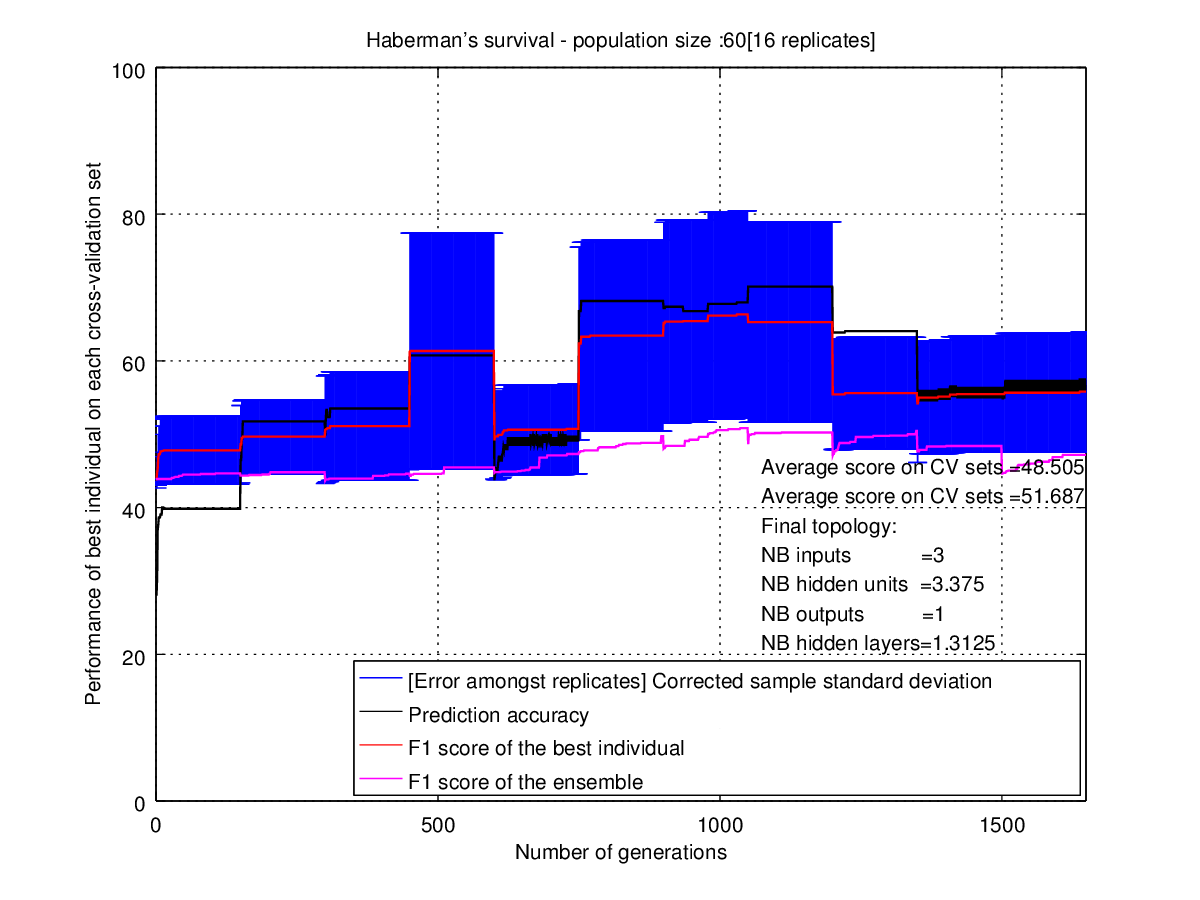
\includegraphics[scale=0.7]{haberman-performancesVSepochs-PSO}
  \vspace{-12pt}
  \caption{Optimization of the neural network population (PSO)}
  \label{haberman-perfs-PSO}
\end{figure}

\begin{figure}[h]
  \centering
  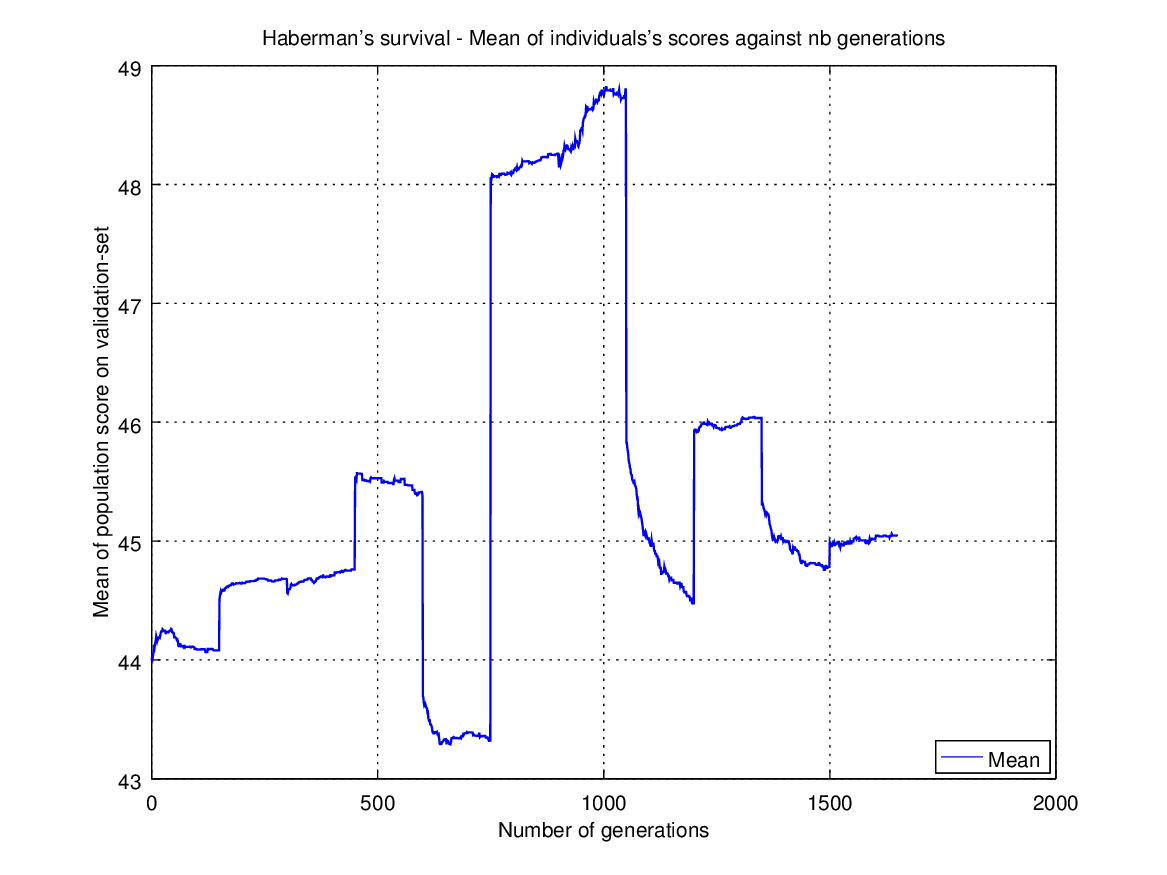
\includegraphics[scale=0.7]{haberman-meanVSepochs-PSO}
  \vspace{-12pt}
  \caption{Mean of the scores of the individuals (PSO)}
  \label{haberman-mean-PSO}
\end{figure}

\clearpage
\bibliography{latex-citations}{}
\bibliographystyle{plain}

\end{document}
